% (c) 2012-2013 Claudio Carboncini - claudio.carboncini@gmail.com
% (c) 2012-2014 Dimitrios Vrettos - d.vrettos@gmail.com

\chapter{Trigonometria}

\section{Prime definizioni}

L'etimologia della parola ``trigonometria'' dal greco $\tau\rho\acute{\iota}\gamma\omega\nu o\nu$ (\emph{trígonon} triangolo) e $\mu\acute{\epsilon}\tau\rho o\nu$ (\emph{métron} misura) chiarisce in cosa consiste
questa parte della matematica che ci accingiamo ad affrontare.
La trigonometria nasce dal problema di ``risolvere un triangolo'', cioè di ricavare la misura di alcuni suoi elementi incogniti date
le misure di altri elementi. Dal momento che gli elementi di un triangolo sono sei, i tre lati e i tre angoli, vedremo come, date le misure di
almeno tre di questi elementi di cui almeno uno sia un lato, sia possibile determinare la misura degli altri tre elementi mancanti.
\begin{multicols}{2}
 Disegniamo un triangolo rettangolo, retto in~$A$, avendo cura di indicare con la stessa lettera vertice (maiuscola) e lato opposto (minuscola), come nella figura a fianco.
Ricordiamo che tra i lati sussiste la relazione del teorema di Pitagora~$\overline{BC}^{2}=\overline{AC}^{2}+\overline{AB}^{2}$ e che ciascun cateto
è minore dell'ipotenusa. Ricordiamo anche che gli angoli acuti sono complementari~$\widehat {C}+\widehat {B}=90\grado$.
\begin{center}\label{fig:triangolo_rettangolo}
 % (c) 2012 Dimitrios Vrettos - d.vrettos@gmail.com

\begin{tikzpicture}[x=15mm,y=15mm, font=\small]

\coordinate (A) at (0,0);
\coordinate (B) at ($(A)+(0:2.5)$);
\coordinate (C) at ($(A)+(90:2)$);
\draw (A) node[below left]{$A$} -- (B) node[below right]{$B$}node[midway,below]{$c$} -- (C)node[above left]{$C$}node[midway,above]{$a$} -- (A)node[midway,left]{$b$};

\tkzMarkAngle[ fill=LimeGreen, draw, size=.3](A,C,B)
\tkzLabelAngle[pos=.5](A,C,B){$\gamma$}

\tkzMarkAngle[ fill=LimeGreen ,draw, size=.3](C,B,A)
\tkzLabelAngle[pos=.6](A,B,C){$\beta$}

\tkzMarkRightAngle[ fill=LimeGreen,draw, size=.2](C,A,B);
\tkzLabelAngle[pos=.4](C,A,B){$\alpha$}

\begin{scope}[fill=CornflowerBlue, draw=black]
\filldraw (0,0) circle (1pt);
\filldraw (0,2) circle (1pt);
\filldraw (2.5,0) circle (1pt);
\end{scope}

\end{tikzpicture}
\end{center}
\end{multicols}
\osservazione Basta conoscere la misura di due lati per determinare la misura del terzo lato, ma queste informazioni non ci permettono di determinare
l'ampiezza degli angoli acuti se non in casi particolari. Se conosciamo un angolo acuto e la misura di un lato non possiamo determinare la misura
degli altri elementi mancanti.

Riferendoci alla figura, chiamiamo cateto adiacente all'angolo acuto~$\beta$ il cateto~${AB}$ indicato con~$c$ e cateto opposto all'angolo~$\beta$ il
cateto~${AC}$ indicato con~$b$.

\begin{definizione}
Con riferimento al triangolo in figura si definiscono le grandezze \emph{seno di $\beta$}, \emph{coseno di $\beta$} e \emph{tangente di $\beta$} rispettivamente
\begin{align*}
&\sin(\beta)=\frac{\text{cateto opposto a }\beta}{\text{ipotenusa}}=\frac{\overline{AC}}{\overline{CB}}=\frac{b}{a}\quad\Rightarrow\quad b=a\cdot \sin(\beta)\\
&\cos(\beta)=\frac{\text{cateto adiacente a }\beta}{\text{ipotenusa}}=\frac{\overline{AB}}{\overline{CB}}=\frac{c}{a}\quad\Rightarrow\quad c=a\cdot \cos(\beta)\\
&\tan(\beta)=\frac{\text{cateto opposto a }\beta}{\text{cateto adiacente a }\beta}=\frac{\overline{AC}}{\overline{AB}}=\frac{b}{c}\quad\Rightarrow\quad b=c\cdot \tan(\beta).
\end{align*}
\end{definizione}

\begin{definizione}
In maniera analoga, per l'angolo~$\gamma$, complementare di $\beta$ ($\gamma =90\grado - \beta$):
\begin{align*}
&\sin(\gamma)=\frac{\text{cateto opposto a }\gamma}{\text{ipotenusa}}=\frac{\overline{AB}}{\overline{CB}}=\frac{c}{a}\quad\Rightarrow\quad c=a\cdot \sin(\gamma)\\
&\cos(\gamma)=\frac{\text{cateto adiacente a }\gamma}{\text{ipotenusa}}=\frac{\overline{AC}}{\overline{CB}}=\frac{b}{a}\quad\Rightarrow\quad b=a\cdot \cos(\gamma)\\
&\tan(\gamma)=\frac{\text{cateto opposto a }\gamma}{\text{cateto adiacente a }\gamma}=\frac{\overline{AB}}{\overline{AC}}=\frac{c}{b}\quad\Rightarrow\quad c=b\cdot \tan(\gamma).
\end{align*}
\end{definizione}

Le definizioni sono ben poste: le funzioni \emph{seno dell'angolo} (sen o~$\sin$), \emph{coseno dell'angolo} ($\cos$), \emph{tangente dell'angolo}
($\tan$ o tg) dipendono solo dall'angolo e non dal particolare triangolo rettangolo usato. Infatti angoli acuti della stessa misura appartengono a
triangoli rettangoli tutti simili tra loro; dato che i lati di triangoli simili sono in proporzione, il rapporto tra i lati è invariato.
Inoltre possiamo certamente affermare che le funzioni seno e coseno di angoli acuti assumono valori positivi minori di~$1$,
poiché in un triangolo rettangolo il cateto è minore dell'ipotenusa.

Dal confronto delle definizioni notiamo che valgono le uguaglianze:
\[\sin(\gamma)=\cos(\beta)\qquad \cos(\gamma)=\sin(\beta)\qquad \tan(\gamma)=\frac{1}{\tan(\beta)}\]
per cui possiamo anche scrivere:
\[\sin(x)=\cos(90\grado-x)\qquad \cos(x)=\sin(90\grado-x)\qquad \tan(x)=\frac{1}{\tan(90\grado-x)}.\]

\begin{exrig}
 \begin{esempio}
Nel triangolo rettangolo~$ABC$ i cateti misurano rispettivamente~$AB=4\unit{m}$, $AC=3\unit{m}$ e l'ipotenusa misura~$5\unit{m}$.
Possiamo determinare le funzioni trigonometriche dei suoi angoli acuti semplicemente applicando le definizioni.
Si ottiene
\[\sin(\beta)=\frac{b}{a}=\frac{3}{5}\text{,}\quad \cos(\beta)=\frac{c}{a}=\frac{4}{5}\text{,}\quad \tan(\beta)=\frac{b}{c}=\frac{3}{4}.\]
Per l'angolo complementare $\gamma$ lasciamo al lettore il completamento:
\[\sin(\gamma)=\ldots\ldots\text{,}\quad \cos(\gamma)=\ldots\ldots\text{,}\quad \tan(\gamma)=\ldots\ldots.\]
 \end{esempio}
\end{exrig}

\osservazione Ancora non possiamo avere informazioni sull'ampiezza degli angoli acuti;
vedremo in seguito come procedere nei calcoli e quindi concludere la risoluzione del triangolo.

\vspace{1.10ex}
\ovalbox{\risolvi \ref{ese:C.1}}

\section{Due identità fondamentali}

Dalle definizioni date nella sezione precedente otteniamo le seguenti identità fondamentali:
\[\tan(\gamma)=\frac{a\cdot \sin(\gamma)}{a\cdot \cos(\gamma)}=\frac{\sin(\gamma)}{\cos(\gamma)}\]
cioè la tangente di un angolo è il rapporto tra il seno dell'angolo e il coseno dello stesso angolo. In generale:
 \begin{equation}
 \label{eq:F.1}
 \tan(x)=\frac{\sin(x)}{\cos(x)}.
 \end{equation}

Dal teorema di Pitagora si ha~$a^{2}=b^{2}+c^{2}$ da cui, dividendo ambo i membri per~$a^{2}$, si ottiene
\begin{align*}
\frac{a^{2}}{a^{2}} &= \frac{b^{2}+c^{2}}{a^{2}}=\frac{b^{2}}{a^{2}}+\frac{c^{2}}{a^{2}}\\
\Rightarrow 1 &= \left(\frac{b}{a}\right)^{2}+\left(\frac{c}{a}\right)^{2}\\
\Rightarrow 1 &= \left(\cos(\gamma)\right)^{2}+\left(\cos (\gamma)\right)^{2}\\
\Rightarrow 1 &= \cos^{2}(\gamma)+\sin^{2}(\gamma).
\end{align*}
In generale, per qualunque angolo~$x$ vale
\begin{equation}
\label{eq:F.2}
 \cos^{2}(x)+\sin^{2}(x)=1.
\end{equation}

\begin{definizione}
Si definiscono inoltre altre funzioni trigonometriche che potranno servire nella risoluzione dei triangoli, la
\emph{secante}, la \emph{cosecante} e la \emph{cotangente} di un angolo $x$, rispettivamente:
\[\sec(x)=\frac{1}{\cos(x)}\qquad\csc(x)=\frac{1}{\sin(x)}\qquad\cot(x)=\frac{1}{\tan(x)}.\]
\end{definizione}

\begin{exrig}
 \begin{esempio}
In un triangolo rettangolo si sa che~$\cos(\beta)=\frac{3}{4}$, determinare~$\sin(\beta)$ e~$\tan(\beta)$.

\emph{Strategia risolutiva:}
ricordando che per qualunque angolo~$x$ vale la~\ref{eq:F.2} possiamo sostituire il dato e calcolare
$\sin(\beta)=\sqrt{1-\cos ^{2}(\beta )}=\sqrt{1-\frac{9}{16}}=\frac{\sqrt{7}}{4}$. Infine, sapendo che per ogni
angolo vale la \ref{eq:F.1}, cioè~$\tan(x)=\frac{\sin(x)}{\cos (x)}$, ricaviamo:
\[\tan(\beta)=\cfrac{\frac{\sqrt{7}}{4}}{\frac{3}{4}}=\frac{\sqrt{7}}{3}.\]

Osserviamo che nella determinazione di~$\sin(\beta)$ abbiamo trascurato il valore negativo in quanto abbiamo definito
le funzioni goniometriche come rapporto delle misure di due segmenti.
 \end{esempio}
\end{exrig}

\ovalbox{\risolvi \ref{ese:C.2}}

\section{Angoli particolari}
Possiamo ricavare per via geometrica il valore esatto delle funzioni trigonometriche di angoli particolari.

\subsection{Angoli di~45°}

 Il triangolo rettangolo isoscele (figura~\ref{fig:C.1}) ha gli angoli acuti di~$45\grado$ ed è la metà di un quadrato di lato~$l$.
Sappiamo che~$d=\sqrt{l^{2}+l^{2}}=\sqrt{2l^2}=\sqrt{2}l$; poiché il calcolo delle funzioni trigonometriche per un angolo
non dipende dal particolare triangolo usato, possiamo concludere per le definizioni date:
$\sin(45\grado)=\frac{l}{\sqrt{2}l}=\frac{1}{\sqrt{2}}=\frac{\sqrt{2}}{2}$ e anche
$\cos(45\grado)=\frac{\sqrt{2}}{2}$ e per la definizione di tangente dell'angolo~$\tan(45\grado)=1$.

\begin{figure}[t]
\begin{minipage}[t]{.45\textwidth}
 \centering
 % (c) 2012 Dimitrios Vrettos - d.vrettos@gmail.com

\begin{tikzpicture}[x=10mm,y=10mm, font=\small]

\coordinate (B) at (0,0);
\coordinate (A) at ($(B)+(0:-2.5)$);
\coordinate (C) at ($(B)+(90:2.5)$);
\draw (A) node[below left]{$A$} -- (B) node[below right]{$B$}node[midway,below]{$l$} -- (C)node[above right]{$C$}node[midway,right]{$l$} -- (A)node[midway,left=0.05]{$d$};

\node[above left]at (-2.5,2.5) {$D$};
\tkzMarkAngle[fill=LimeGreen, draw, size=.3](B,A,C)
\tkzMarkAngle[fill=LimeGreen, draw, size=.3](A,C,B)
\tkzMarkRightAngle[fill=LimeGreen,draw, size=.2](A,B,C)


\tkzLabelAngle[pos=1, below=-0.1](C,A,B){$\alpha=45\grado$}
\tkzLabelAngle[pos=0.55](A,C,B){$\alpha$}
\begin{scope}[fill=CornflowerBlue, draw=black]
\filldraw (0,0) circle (1pt);
\filldraw (0,2.5) circle (1pt);
\filldraw (-2.5,0) circle (1pt);
\filldraw (-2.5,2.5) circle (1pt);
\end{scope}

\begin{scope}[dotted]
\draw (-2.5,0) -- (-2.5,2.5)-- (0,2.5);
\end{scope}

\end{tikzpicture}
 \caption{T.rettangolo isoscele.}\label{fig:C.1}
\end{minipage}\hfil
\begin{minipage}[t]{.45\textwidth}
 \centering
 % (c) 2012 Dimitrios Vrettos - d.vrettos@gmail.com

\begin{tikzpicture}[x=10mm,y=10mm, font=\small]
  \coordinate (H) at (0,0);
  \coordinate (A) at ($(H)+(90:2.6)$);
  \coordinate (C) at ($(H)+(0:1.3)$);
  \coordinate (B) at ($(H)+(0:-1.3)$);
  \draw (A) node[above]{$A$} -- (B) node[below left]{$B$}node[midway,left]{$l$} -- (H)node[below]{$H$}node[midway,below]{$\frac{l}{2}$}  -- (A)node[midway,left]{$h$}-- (C)node[below right]{$C$}node[midway,right]{$l$} -- (H)node[midway,below]{$\frac{l}{2}$};

  \tkzMarkAngle[ fill=LimeGreen ,draw, size=.4](H,A,C)
  \tkzMarkAngle[ fill=LimeGreen ,draw, size=.3](A,C,H)
  \tkzMarkRightAngle[fill=LimeGreen,draw, size=.2](A,H,C)
  
  \begin{scope}[font=\scriptsize]
    \tkzLabelAngle[pos=.9](C,A,H){$30\grado$}
    \tkzLabelAngle[pos=.5](H,C,A){$60\grado$}
    \tkzLabelAngle[pos=.5](A,H,C){$90\grado$}
  \end{scope}

  \begin{scope}[fill=CornflowerBlue, draw=black]
    \filldraw (0,0) circle (1pt);
    \filldraw (0,2.6) circle (1pt);
    \filldraw (-1.3,0) circle (1pt);
    \filldraw (1.3,0) circle (1pt);
  \end{scope}

\end{tikzpicture}
 \caption{T.rettangolo con angoli di~$30\grado$ e~$60\grado$.}\label{fig:C.2}
\end{minipage}
\end{figure}

\subsection{Angoli di~30° e~60°}

Il triangolo rettangolo con un angolo di~$30\grado$ ha l'altro angolo acuto di~$60\grado$ (figura~\ref{fig:C.2}) pertanto possiamo trattare insieme
la ricerca delle funzioni trigonometriche di tali angoli.

Il triangolo rettangolo in questione è la metà di un triangolo equilatero di lato~$l$ e altezza~$h$; poiché $\overline{HC}$ è metà del lato
possiamo subito dire che~$\cos(60\grado)=\frac{\overline{HC}}{l}=\frac{l/2}{l}=\frac{1}{2}$.
Per le definizioni date si ha~$\sin(60\grado)=\frac{\overline{AH}}{l}$.
Applicando il teorema di Pitagora si ottiene
\[\overline{AH}=\sqrt{l^{2}-\left(\frac{l}{2}\right)^{2}}=\sqrt{l^2-\frac{l^2}{4}}=
\sqrt{\frac{3}{4}}l=\frac{\sqrt{3}}{\sqrt{4}}l=\frac{\sqrt{3}}{2}l
\quad\Rightarrow\quad\sin(60\grado)=\frac{\sqrt{3}}{2}.\]
Infine~$\tan(60\grado)=\dfrac{\sin(60\grado)}{\cos(60\grado)}=\sqrt{3}$.

Ricordando che per angoli complementari è~$\sin(x)=\cos(90\grado-x)$ e~$\cos(x)=\sin(90\grado-x)$
ed essendo~$30\grado=90\grado-60\grado$ possiamo scrivere:
\[\sin(30\grado)=\cos(60\grado)=\frac{1}{2};\qquad\cos(30\grado)=\sin(60\grado)=\frac{\sqrt{3}}{2}\]
e infine
\[\tan(30\grado)=\cfrac{\frac{1}{2}}{\frac{\sqrt{3}}{2}}=\frac{1}{\sqrt{3}}=\frac{\sqrt{3}}{3}.\]%[figura~4]

\subsection{Angoli di~0° e~90°}

Ovviamente non esiste un triangolo con un angolo di~$0\grado$: si tratta di un triangolo che degenera in un segmento.
Possiamo pensare ad un triangolo rettangolo come nella figura di pagina~\pageref{fig:triangolo_rettangolo}, avente~$a=1$ e immaginare di muovere il vertice~$C$ in modo da rimpicciolire
sempre più l'angolo~$\beta$; quando~$\beta$ diventa~$0\grado$ il segmento~$b$ si riduce ad un punto e si ha
$b=0$ e quindi~$sin(0\grado)=0$, l'ipotenusa~$a$ coincide con il cateto~$c$ quindi~$\cos(0\grado)=1$ e infine~$\tan(0\grado)=0$.

Allo stesso modo, se deformiamo il triangolo fino ad avere l'angolo~$\gamma$ di~$0\grado$, quindi~$\beta$ di~$90\grado$, otteniamo
che~$\sin(90\grado)=1$ e~$\cos(90\grado)=0$; applicando la formula della tangente si avrà una frazione con denominatore nullo e
quindi diremo che~$\tan(90\grado)$ non è definita.

Possiamo riassumere i valori trovati per questi angoli particolari in una tabella:
\[
\begin{array}{cccc}
\toprule
\text{angolo}\, x & \sin(x)&\cos(x) & \tan(x)\\
\midrule
0\grado & 0 & 1 & 0\\[2pt]
30\grado & \dfrac{1}{2} & \dfrac{\sqrt{3}}{2} & \dfrac{\sqrt{3}}{3}\\[8pt]
45\grado & \dfrac{\sqrt{2}}{2} & \dfrac{\sqrt{2}}{2} & 1\\[8pt]
60\grado & \dfrac{\sqrt{3}}{2} & \dfrac{1}{2} & \sqrt{3}\\[7pt]
90\grado & 1 & 0 & \text{non definita}\\
\bottomrule
\end{array}
\]

Come possiamo ottenere i valori delle funzioni trigonometriche per angoli diversi da quelli sopra considerati?

\section{Usare la calcolatrice}

Sul mercato ci sono vari tipi di calcolatrice scientifica, ciascuno dovrà familiarizzare con la propria calcolatrice per imparare
ad impostare correttamente il calcolo da effettuare e i tasti da pigiare per ottenere il corretto risultato. Se non si digita in
modo consapevole e se non si sanno leggere i risultati, la calcolatrice è uno strumento inutilizzabile e talvolta può anche essere dannoso.

Nel seguito faremo riferimento alla calcolatrice \emph{kcalc} (figura~\ref{fig:C.4}), in dotazione all'ambiente di desktop \emph{KDE}\footnote{K Desktop Environment (\url{http://it.wikipedia.org/wiki/KDE}).} (\emph{GNU/Linux}\footnote{un sistema operativo per computer (\url{http://it.wikipedia.org/wiki/Linux}).}), cercando di dare
riferimenti che si adattino a tutte le calcolatrici.

\paragraph{Passo I: scelta dell'unità di misura}

Sicuramente conosci già, come unità di misura degli angoli, il \emph{grado sessagesimale} (indicato con il simbolo $\grado$). Esistono però altre unità di misura utilizzate in contesti diversi:
i \emph{gradi centesimali} (chiamati anche \emph{gradienti}), utilizzati principalmente in topografia, e i \emph{radianti}, utilizzati in matematica, specialmente in analisi.
Su tutte le calcolatrici scientifiche è possibile effettuare le operazioni sugli angoli scegliendo l'opportuna unità di misura:

\begin{center}
\begin{tabular}{lcc}
\toprule
Angolo & Sigla & Sigla abbreviata \\
\midrule
gradi sessagesimali & DEG & $\grado$ \\
gradi centesimali & GRAD & G \\
radianti & RAD & \\
\bottomrule
\end{tabular}
\end{center}

Impostiamo la calcolatrice in modo da ricevere in ingresso angoli misurati in gradi sessagesimali (con \emph{kcalc} dobbiamo impostare il selettore in alto a sinistra sulla pulsantiera sul simbolo $\grado$, altre calcolatrici hanno un pulsante che permette di passare da una impostazione all'altra, in sequenza).

\paragraph{Passo II: calcolo del coseno di un angolo}

Ci proponiamo di determinare~$\cos(60\grado)$.

Controllate di aver impostato l'input dell'angolo in gradi sessagesimali, quindi
digitate~$60$ e premete il tasto \emph{cos}. La calcolatrice restituisce~$0.5$.
Dunque~$\cos(60\grado)=0,5$.

\emph{Attenzione}: per i numeri decimali sulla calcolatrice useremo il ``punto decimale'' in sostituzione della virgola.

\osservazione
\begin{enumeratea}
\item La funzione coseno calcolata su angoli compresi fra~$0\grado$ e~$90\grado$ restituisce sempre numeri compresi fra~$0$ e~$1$.
\item Il coseno vale~$1$ (il massimo) quando l'angolo di input è~$0\grado$ e decresce fino a~$0$ man mano che l'angolo immesso cresce fino
   a~$90\grado$. Detto in altre parole: il coseno di un angolo che cresce da~$0\grado$ a~$90\grado$ diminuisce dal valore~$1$ al valore~$0$.
\item La decrescita del coseno non è proporzionale all'aumento dell'angolo, tant'è vero che si ha:~$\cos(30\grado)=0,867$
   ma~$\cos(60\grado)=0,5$ che non è la metà di~$\cos(30\grado)$.
\end{enumeratea}


\begin{problema}
Il segmento~${AB}$ della figura~\ref{fig:C.3} misura~$5\unit{m}$ e la sua proiezione~${AH}$ sulla retta~$r$ misura~$3\unit{m}$.
Possiamo determinare la misura dell'angolo~${\alpha}$ compreso tra~$r$ e il segmento~${AB}$?

\end{problema}
\begin{figure}[t]
\begin{minipage}[t]{.45\textwidth}
 \centering
 % (c) 2012 Dimitrios Vrettos - d.vrettos@gmail.com

\begin{tikzpicture}[x=10mm,y=10mm, font=\small]
  \coordinate (A) at (0,0);
  \coordinate (H) at ($(A)+(0:3)$);
  \coordinate (B) at ($(H)+(90:4)$);
  \draw(-.5,0)--(3.5,0) node[below right] {$r$};
  
  \draw (B)node[above right]{$B$} --(A) node[below left]{$A$} -- (H) node[below right]{$H$};
  \draw[dashed] (B) -- (H);

  \tkzMarkAngle[fill=LimeGreen ,draw, size=.4](H,A,B)
  \begin{scope}[font=\scriptsize]
  \tkzLabelAngle[pos=.6](H,A,B){$\alpha$}
  \end{scope}
  
  \begin{scope}[fill=CornflowerBlue, draw=black]
    \filldraw (0,0) circle (1pt);
    \filldraw (3,0) circle (1pt);
    \filldraw (3,4) circle (1pt);
  \end{scope}
\end{tikzpicture}
  \caption{$AB$ e la proiezione~${AH}$ su~$r$.}\label{fig:C.3}
\end{minipage}\hfil
\begin{minipage}[t]{.45\textwidth}
 \centering
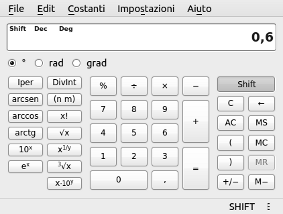
\includegraphics[scale=.60]{/part06/chapC/kcalc.png}
 \caption{Calcolatrice \emph{kcalc}.}\label{fig:C.4}
\end{minipage}
\end{figure}

\emph{Dati}:~$\overline{AB}=5\unit{m}$;\quad~$\overline{AH}=3\unit{m}$. \qquad\emph{Obiettivo}:~$\alpha$.

\begin{soluzione}
 Partiamo dalla formula~$\overline{AH}=\overline{AB}\cdot \cos(\alpha)$, da essa possiamo ottenere
$\cos(\alpha)=\frac{\overline{AH}}{\overline{AB}}$. Sostituendo i valori noti otteniamo
$\cos(\alpha)=\frac{\overline{AH}}{\overline{AB}}=\frac{3}{5}=\np{0,6}$.

Per risalire dal valore del coseno al valore dell'angolo usiamo la calcolatrice attivando la funzione inversa di coseno; su molte calcolatrici
tale funzione è indicata con~$\cos^{-1}$, funzione che si attiva premendo il tasto \emph{Shift} (figura~\ref{fig:C.4}); in \emph{kcalc}
premendo il tasto \emph{Shift} il tasto $cos$ cambia funzionalità e assumendo quella della sua funzione inversa con la scritta \emph{arccos}.

Calcoliamo la misura dell'angolo il cui coseno è~$0,6$ immettendo tale valore nella calcolatrice e attivando i tasti \emph{Shift} e \emph{arccos}.
La calcolatrice restituisce~$53.13010235$.
Questo risultato ci dice che l'angolo è di~$53\grado$ più una parte decimale~$\np{0,13010235}$.
Ricordiamo che i sottomultipli del grado vengono espressi in sessantesimi ($1\grado=60'$ cioè 60 \emph{primi}),
a loro volta suddivisi in sessantesimi ($1'=60''$ cioè 60 \emph{secondi}).
Dunque la parte decimale estratta dalla calcolatrice va adeguatamente modificata:
al risultato della calcolatrice togliamo la parte intera~$(53)$ e moltiplichiamo per~$60$ ottenendo~$\np{7,806141}$ la cui parte
intera (7) rappresenta i \emph{primi}; togliamo nuovamente la parte intera (7) e moltiplichiamo per~$60$ ottenendo i \emph{secondi}~$\np{48,36846}$
Arrotondiamo la parte intera e possiamo concludere~$\alpha\simeq 53\grado 7'48''$.
Alcune calcolatrici scientifiche fanno in automatico questi calcoli attivando un tasto opportuno.

Osserviamo che viene utilizzato il simbolo~$\simeq$ (circa uguale) per indicare che abbiamo usato valori approssimati.
Ora sei in grado di determinare l'ampiezza degli angoli acuti attivando le funzioni inverse sulla tua calcolatrice.
\end{soluzione}

\ovalbox{\risolvii \ref{ese:C.3}, \ref{ese:C.4}, \ref{ese:C.5}}

\section{Operazioni con i gradi sessagesimali}

Accenniamo alle addizioni e sottrazioni tra angoli.

\begin{exrig}
 \begin{esempio}
Svolgiamo l'operazione~$48\grado~45' 52'' + 62\grado~27' 22''$.
\begin{center}
 % (c) 2012 Dimitrios Vrettos - d.vrettos@gmail.com

\begin{tikzpicture}[x=10mm,y=10mm]

\matrix (a) [matrix of nodes,matrix anchor=east] at (0,0){
48$\grado$&45'&52''&$+$\\
62$\grado$&27'&22''&{}\\
110$\grado$&72'&74''&{}\\
111$\grado$&13'&14''&{}\\};

\draw (a-2-1.south west) -- (a-2-4.south east);
\end{tikzpicture}
\end{center}

Sommando termine a termine otteniamo~$110\grado~72' 74''$. Tenendo conto che~1 grado equivale a~60 primi e~1 primo equivale a~60 secondi,
si ha che i~$74\grado$ valgono~$1'$ e~$14''$, i~$72' 74''$ diventano allora~$73'$ e~$14''$.
Trasformiamo poi i~$73'$ in~$1\grado$ e~$13'$.

In definitiva si ha che~$110\grado~72' 74'' = 111\grado~13' 14''$.
 \end{esempio}

 \begin{esempio}
Svolgiamo ora una sottrazione:~$90\grado - 45\grado~33' 12''$.
\begin{center}
 % (c) 2012 Dimitrios Vrettos - d.vrettos@gmail.com

\begin{tikzpicture}[x=10mm,y=10mm]

\matrix (a) [matrix of nodes,matrix anchor=north] at (0,0){
90$\grado$&&&$-$\\
45$\grado$&33'&12''&{}\\};

\draw (a-2-1.south west) -- (a-2-3.south east);

\begin{scope}[xshift=14mm,yshift=-10mm,->, Maroon, thick]
\draw (0,0) -- (.5,0);
\end{scope}

\begin{scope}[xshift=35mm]
\matrix (a) [matrix of nodes,matrix anchor=north] at (0,0){
89$\grado$&59'&60''&$-$\\
45$\grado$&33'&12''&{}\\
44$\grado$&26'&48''&{}\\};

\draw (a-2-1.south west) -- (a-2-3.south east);
\end{scope}
\end{tikzpicture}
\end{center}

Questa è una operazione molto comune, poiché capita abbastanza spesso di dover calcolare l'angolo complementare.
Per svolgere la sottrazione conviene scrivere~$90\grado$ come~$89\grado~59' 60''$ e svolgere la sottrazione avendo come risultato~$44\grado~26' 48''$.
 \end{esempio}

 \begin{esempio}
Un'ultima sottrazione:~$72\grado~20' 40'' - 23\grado~40' 52''$.

Per fare questa sottrazione parto dai secondi e non potendo fare~$40-52$, utilizzo il riporto trasformando~$72\grado~20' 40''$
in~$72\grado~19' 100''$. Ora posso eseguire agevolmente la sottrazione e ottengo~$100-52=48$;
sottraggo poi i primi tra loro, aggiungendo il riporto ai~$19'$ ($72\grado 19' \:\rightarrow\: 71\grado 79'$) e ottengo~$79-40=39$; sottraggo poi i gradi:~$71-23=48$.
Il risultato finale è quindi~$48\grado~39' 48''$.
 \end{esempio}
\end{exrig}

\ovalbox{\risolvi \ref{ese:C.6}}

\section{Risoluzione di triangoli rettangoli}

Ricordiamo che risolvere un triangolo significa ricavare le misure di tutti i suoi elementi (lati e angoli) date le misure di alcuni di essi.

\begin{exrig}
 \begin{esempio}
Determinate l'area del triangolo rettangolo $ABC$, retto in $A$, sapendo che il cateto~${BC}=2\unit{m}$ e che $\widehat{ABC}=\beta=20\grado$.

\emph{Dati}:~$\widehat{BAC}=90\grado$,\quad~$\overline{BC}=2\unit{m}$,\quad~$\widehat{ABC}=\beta=20\grado$.

\emph{Obiettivo}:~$\Area{(ABC)}$.

\emph{Procedura risolutiva}:
$\Area{(ABC)}=\frac{1}{2}\cdot \overline{AB}\cdot \overline{AC}$.

Dobbiamo dunque determinare le misure dei cateti. Applicando le definizioni ($\gamma=\widehat{ACB}$):
\[\overline{AB}=\overline{BC}\cdot {\cos(\beta)}=2\cdot {\cos(20\grado)}\simeq 2\cdot 0,940\simeq 1,879\]
\[\overline{AC}=\overline{BC}\cdot {\cos(\gamma)}=2\cdot {\cos(70\grado)}\simeq 2\cdot 0,342\simeq 0,684\]

Pertanto $\Area\simeq 0,643\unit{(m^{2})}$.
 \end{esempio}

 \begin{esempio}
Un triangolo rettangolo $ABC$, retto in $A$, ha il cateto~$AB$ di~$5\unit{cm}$ e l'angolo acuto in~$C$ di~$57\grado$; determinate l'altro angolo acuto,
la misura del cateto~$AC$ e la misura dell'ipotenusa~$BC$.

\emph{Dati}:~$\widehat{BAC}=90\grado$,\quad~$\widehat{BCA}=57\grado$,\quad~$\overline{AB}=5\unit{cm}$.

\emph{Obiettivo}:~$\beta=\widehat{ABC}$,\quad~$\overline{AC}$,\quad~$\overline{BC}$.

\emph{Procedura risolutiva}:
Essendo gli angoli acuti complementari si ottiene~$\beta=90\grado-57\grado=33\grado$.
Applicando la formula inversa:
\[\overline{CB}=\frac{\overline{AB}}{\cos(\beta)}=\frac{5}{\cos(33\grado)}\simeq \frac{5}{0,839}\simeq 5,962\unit{cm}.\]
Infine determiniamo l'altro cateto e osserviamo che possiamo procedere in due modi:
\begin{itemize*}
 \item con il Teorema di Pitagora:
 \[\overline{CA}=\sqrt{\overline{CB}^{2}-\overline{AB}^{2}}\simeq \sqrt{35,543-25}\simeq \sqrt{10,543}\simeq 3,247\unit{cm};\]
 \item per definizione di coseno:
 \[\overline{CA}=\overline{CB}\cdot \cos(\gamma)\simeq 5,962 \cdot \cos(57\grado)\simeq 5,962\cdot 0,545\simeq 3,247\unit{cm}.\]
\end{itemize*}
\osservazione
\begin{enumeratea}
\item Nei calcoli effettuati abbiamo operato un'approssimazione; per esempio il valore esatto di~$\overline{CB}$ è rappresentato solo
dall'espressione~$\overline{CB}=\frac{\overline{AB}}{\cos(\beta)}=\frac{5}{\cos(33\grado)}$.
\item I risultati ottenuti con procedimenti diversi possono differire, se pur di poco, a causa dell'uso di valori approssimati
nei calcoli che aumentano l'errore di approssimazione (propagazione dell'errore).
\end{enumeratea}
 \end{esempio}

 \begin{esempio}
Risolvi il triangolo rettangolo della figura sapendo che~$c=20\unit{cm}$ e~$\sin(\beta)=\frac{3}{5}$.
\begin{center}
 % (c) 2012 Dimitrios Vrettos - d.vrettos@gmail.com

\begin{tikzpicture}[x=9mm,y=9mm, font=\small]

  \coordinate (A) at (0,0);
  \coordinate (C) at ($(A)+(90:3)$);
  \coordinate (B) at ($(A)+(0:4)$);

  \draw (A) node[below left]{$A$}-- (C) node[above left]{$C$} -- (B)node[below right]{$B$} -- (A);

  \tkzMarkAngle[ fill=LimeGreen ,draw, size=.4](A,C,B)
  \tkzMarkAngle[ fill=LimeGreen ,draw, size=.4](C,B,A)
  \tkzMarkRightAngle[ fill=LimeGreen ,draw, size=.3](C,A,B)
  
  \begin{scope}[font=\scriptsize]
    \tkzLabelAngle[pos=.6](A,C,B){$\gamma$}
    \tkzLabelAngle[pos=.6](C,B,A){$\beta$}
    \tkzLabelAngle[pos=.6](C,A,B){$\alpha$}
  \end{scope}

  \tkzLabelSegment[midway, left](A,C){$b$}
  \tkzLabelSegment[midway, below](A,B){$c$}
  \tkzLabelSegment[midway, above](B,C){$a$}

  \begin{scope}[fill=CornflowerBlue, draw=black]
    \filldraw (0,0) circle (1pt);
    \filldraw (4,0) circle (1pt);
    \filldraw (0,3) circle (1pt);
  \end{scope}

\end{tikzpicture}
\end{center}
Usiamo l'identità fondamentale per determinare~$\cos(\beta)$:
\[\cos(\beta)=\sqrt{1-\sin^{2}(\beta)}=\sqrt{1-\left(\frac{3}{5}\right)^{2}}=\sqrt{1-\frac{9}{25}}=
    \sqrt{\frac{25-9}{25}}=\sqrt{\frac{16}{25}}=\frac{4}{5};\]

Poiché $\cos(\beta)=\dfrac{c}{a}$ si ha:
\[a=\frac{c}{\cos(\beta)}=\frac{20}{\frac{4}{5}}=\frac{20\cdot{5}}{4}=25\unit{cm}.\]

Per il teorema di Pitagora~$b=\sqrt{a^{2}-c^{2}}=\sqrt{25^{2}-20^{2}}=15\unit{cm}$;

$\beta\simeq 36\grado~52' 12''$ (calcolato con la calcolatrice e arrotondato), $\gamma = 90\grado - \beta \simeq 53\grado~07'48''$.
 \end{esempio}

 \begin{esempio}
Risolvere il triangolo rettangolo~$ABC$, retto in~$A$ (quello della figura precedente) sapendo che~$b=2\unit{cm}$ e~$\sin(\beta)=0,2$.

\emph{Dati}:~$b=2\unit{cm}$,\quad~$\sin(\beta)=0,2$.

\emph{Obiettivo}:~$a$,\quad~$c$,\quad~${\beta}$,\quad~${\gamma}$.

\emph{Procedura risolutiva}:
Dalle definizione di seno $\sin(\beta)=\dfrac{b}{a}$ si ha
\[a=\frac{b}{\sin(\beta)}=\frac{2}{0,2}=10\unit{cm}.\]
Con il teorema di Pitagora possiamo ricavare l'altro cateto
\[c=\sqrt{a^{2}-b^{2}}=\sqrt{100-4}=\sqrt{96}=4\sqrt{6}\simeq 9,798\unit{cm}.\]
Infine, con la funzione inversa, ricaviamo l'angolo~${\beta}=\sin^{-1}(0,2)\simeq 11,537$ e procedendo come spiegato in
precedenza otteniamo:~${\beta}\simeq 11\grado~32' 13''$ e~${\gamma}=90\grado-\beta\simeq 78\grado~27'47''$.
 \end{esempio}
\end{exrig}

\ovalbox{\risolvii \ref{ese:C.7}, \ref{ese:C.8}, \ref{ese:C.9}, \ref{ese:C.10}}

\subsection{Proiezione di un segmento lungo una direzione}

\begin{definizione}
Dato un segmento~$AB$ ed una retta~$r$ che passa per un suo estremo ($A$, per fissare le idee). Si definisce
\emph{proiezione del segmento $AB$ sulla retta $r$} il segmento~$AH$ dove~$H$ è l'intersezione fra~$r$ e la
sua perpendicolare passante per~$B$ (si vedano i tre esempi riportati nella figura seguente).
\end{definizione}

\begin{center}
 % (c) 2012 Dimitrios Vrettos - d.vrettos@gmail.com

\begin{tikzpicture}[x=10mm,y=10mm, font=\small]

  \coordinate (A) at (0,0);
  \coordinate (H) at ($(A)+(0:3)$);
  \coordinate (B) at ($(H)+(90:2)$);

  \draw (B)node[above right]{$B$} -- (A) node[below]{$A$}-- (H) node[below]{$H$};
  \draw[dashed] (B)--(H);

  \draw (-.5,0) -- (3.5,0)node[below] {$r$};
  \tkzMarkAngle[ fill=LimeGreen ,draw, size=.4](H,A,B)

  \begin{scope}[font=\scriptsize]
    \tkzLabelAngle[pos=.6](H,A,B){$\alpha$}
  \end{scope}

  \begin{scope}[fill=CornflowerBlue, draw=black]
    \filldraw (0,0) circle (1pt);
    \filldraw (3,0) circle (1pt);
    \filldraw (3,2) circle (1pt);
  \end{scope}

  \begin{scope}[xshift=45mm]
    \tkzDefPoints{0/1/A, 2/0/B,1.25/1.59/H}
    \tkzDrawLine[add=0 and 0, dashed, thin](B,H)
    \tkzDrawLine[add=0 and 0,thin](A,B)
    \tkzMarkAngle[fill=LimeGreen ,draw, size=.4](B,A,H) 
    \tkzDrawLine[add = .4 and .4, end=$r$, thin](A,H)

    \tkzLabelPoint[above](H){$H$}
    \tkzLabelPoint[above](A){$A$}
    \tkzLabelPoint[below](B){$B$}
    
    \begin{scope}[font=\scriptsize]
      \tkzLabelAngle[pos=.6](H,A,B){$\alpha$}
    \end{scope}
    
    \tkzDrawPoints[fill=CornflowerBlue](A,B, H)
  \end{scope}

  \begin{scope}[xshift=80mm, rotate=-10]
    \tkzDefPoints{0/0/A, 0/2/H, 2/2/B}
    \tkzDrawLine[add=0 and 0, dashed, thin](B,H)
    \tkzDrawLine[add=0 and 0,thin](A,B)
    \tkzDrawLine[add = 0 and .2, end=$r$, thin](A,H)

    \tkzLabelPoint[left](H){$H$}
    \tkzLabelPoint[below](A){$A$}
    \tkzLabelPoint[right](B){$B$}
    \tkzMarkAngle[fill=LimeGreen ,draw, size=.4](B,A,H) 

  \begin{scope}[font=\scriptsize]
    \tkzLabelAngle[pos=.6](H,A,B){$\alpha$}
  \end{scope}
    \tkzDrawPoints[fill=CornflowerBlue](A,B, H)
  \end{scope}
\end{tikzpicture}
\end{center}

\ovalbox{\risolvii \ref{ese:C.11}, \ref{ese:C.12}, \ref{ese:C.13}, \ref{ese:C.14}, \ref{ese:C.15}, \ref{ese:C.16}, \ref{ese:C.17}, \ref{ese:C.18},
\ref{ese:C.19}, \ref{ese:C.20}, \ref{ese:C.21}}

\section{Risoluzione di un triangolo qualsiasi con triangoli rettangoli}
Per risolvere i triangoli qualsiasi, tramite l'altezza, bisogna ricercare all'interno della figura considerata dei triangoli rettangoli.
Nel seguito saranno indicati altri teoremi che permettono
di risolvere tutti i tipi di triangoli.

\begin{figure}[b]
\begin{minipage}[t]{.45\textwidth}
 \centering
 % (c) 2012 Dimitrios Vrettos - d.vrettos@gmail.com

\begin{tikzpicture}[x=10mm,y=10mm, font=\small]

  \coordinate (A) at (0,0);
  \coordinate (B) at ($(A)+(0:4.18)$);
  \coordinate (C) at ($(A)+(39:3.5)$);
  \coordinate (H) at ($(A)+(0:2.72)$);

  \draw (B) node[below right]{$B$}--(A) node[below left]{$A$}--(C) node[above]{$C$}--(B);

  \tkzMarkAngle[ fill=LimeGreen ,draw, size=.4](H,A,C)
  \tkzMarkAngle[ fill=LimeGreen ,draw, size=.4](A,C,B)
  \tkzMarkAngle[ fill=LimeGreen ,draw, size=.4](C,B,H)

  \draw (C)--(H) node[below]{$H$};

  \begin{scope}[font=\scriptsize]
    \tkzLabelAngle[pos=.6](H,A,C){$\alpha$}
    \tkzLabelAngle[left, pos=.6](A,C,B){$\gamma$}
    \tkzLabelAngle[pos=.6](C,B,H){$\beta$}
  \end{scope}
  
  \begin{scope}[fill=CornflowerBlue, draw=black]
    \filldraw (0,0) circle (1pt);
    \filldraw (4.18,0) circle (1pt);
    \filldraw (2.72,2.2) circle (1pt);
    \filldraw (2.72,0) circle (1pt);
  \end{scope}
\end{tikzpicture}
 \caption{Triangolo acutangolo.}\label{fig:C.5}
\end{minipage}\hfil
\begin{minipage}[t]{.45\textwidth}
\centering
 % (c) 2012 Dimitrios Vrettos - d.vrettos@gmail.com

\begin{tikzpicture}[x=10mm,y=10mm, font=\small]

  \coordinate (A) at (0,0);
  \coordinate (B) at ($(A)+(0:4.26)$);
  \coordinate (C) at ($(B)+(145:3.486)$);
  \coordinate (D) at ($(A)+(90:2)$);

  \draw (D) node[above left]{$D$}--(A) node[below left]{$A$}--(B) node[below right]{$B$}--(C)node [above right]{$C$} --(D);

  \tkzMarkAngle[ fill=LimeGreen ,draw, size=.4](C,A,D)
  \tkzMarkAngle[ fill=LimeGreen ,draw, size=.4](A,C,B)
  \tkzMarkAngle[ fill=LimeGreen ,draw, size=.4](C,B,A)

  \draw[dashed] (C)--(A);

  \begin{scope}[fill=CornflowerBlue, draw=black]
    \filldraw (0,0) circle (1pt);
    \filldraw (4.26,0) circle (1pt);
    \filldraw (1.4,2) circle (1pt);
    \filldraw (0,2) circle (1pt);
  \end{scope}
\end{tikzpicture}
\caption{Trapezio rettangolo.}\label{fig:C.6}
\end{minipage}
 \end{figure}

\begin{exrig}
 \begin{esempio}
Risolvi il triangolo acutangolo della figura~\ref{fig:C.5} con~$\alpha=39\grado$, $\beta=57\grado$ e $\overline{CH}=11\unit{m}$.

Ricordando che la somma degli angoli di un triangolo è~$180\grado$ ricaviamo~$\gamma$:
\[ \gamma =180\grado-\alpha -\beta =180\grado-39\grado-57\grado=84\grado.\]

Individuiamo ora i triangoli rettangoli nella figura in modo da poter applicare le formule.

Con il triangolo rettangolo~$CHB$:
\begin{align*}
 &\sin(\beta)=\frac{\overline{CH}}{\overline{CB}} \quad\Rightarrow\quad \overline{CB}=\frac{\overline{CH}}{\sin(\beta)}=
    \frac{11}{\sin(57\grado)}\simeq \np[m]{13,2};\\
&\tan(\beta)=\frac{\overline{CH}}{\overline{BH}} \quad\Rightarrow\quad \overline{BH}=\frac{\overline{CH}}{\tan(\beta)}=
    \frac{11}{\tan(57\grado)}\simeq \np[m]{7,15}.
\end{align*}

Con il triangolo rettangolo~$AHC$:
\begin{align*}
&\sin(\alpha)=\frac{\overline{CH}}{\overline{AC}} \quad\Rightarrow\quad \overline{AC}=\frac{\overline{CH}}{\sin(\alpha)}=
    \frac{11}{\sin(39\grado)}\simeq \np[m]{17,46};\\
&\tan(\alpha)=\frac{\overline{CH}}{\overline{AH}} \quad\Rightarrow\quad \overline{AH}=\frac{\overline{CH}}{\tan(\beta)}=
    \frac{11}{\tan(39\grado)}\simeq \np[m]{13,75}.
\end{align*}

Infine calcoliamo~$\overline{AB}=\overline{AH}+\overline{BH}\simeq \np{7,15}+\np{13,75} = \np{20,9}\unit{m}$.
 \end{esempio}
\end{exrig}

\ovalbox{\risolvii \ref{ese:C.22}, \ref{ese:C.23}, \ref{ese:C.24}, \ref{ese:C.25}}

\subsection{Quadrilateri}

\begin{exrig}\vspace{1.10ex}
 \begin{esempio}
Nel trapezio rettangolo~$ABCD$ della figura~\ref{fig:C.6} il lato obliquo~$BC$ forma un angolo di~$35\grado$ con la base maggiore~$AB$, inoltre la diagonale~$AC$
è perpendicolare a~$BC$. Calcola il perimetro e l'area del trapezio sapendo che la sua altezza è~$10\unit{cm}$.

Ricordando che la somma degli angoli di un triangolo è~$180\grado$ ricaviamo~$\widehat{CAB}=55\grado$.
Siccome il trapezio è rettangolo
$\widehat{DAC}=\widehat{DAB}-\widehat{CAB}=90\grado-55\grado$.
Calcoliamo ora~$CB$, $AB$ e~$DC$:
\begin{align*}
&\sin(\widehat{ABC})=\frac{\overline{AD}}{\overline{CB}} \quad\Rightarrow\quad
    \overline{CB}=\frac{\overline{AD}}{\sin(\widehat{ABC})}=\frac{10}{\sin(35\grado)}\simeq \np[cm]{17,43};\\
&\overline{AB}=\frac{\overline{CB}}{\cos(\widehat{ABC})}\simeq \frac{\np{17,43}}{\cos(55\grado)}\simeq \np[cm]{21,28};\\
&\frac{\overline{DC}}{\overline{AD}}=\tan(\widehat{DAC}) \quad\Rightarrow\quad \overline{DC}=\overline{AD}\cdot\tan(\widehat{DAC})=10\tan(35\grado)\simeq \np{7,00}.
\end{align*}

Da cui:
\begin{align*}
&2p=\overline{AB}+\overline{BC}+\overline{DC}+\overline{DA}\simeq \np{21,28}+\np{17,43}+\np{7,00}+10 = \np[cm]{55,71};\\
&\Area=\frac{(\overline{AB}+\overline{DC})\cdot\overline{AD}}{2}\simeq \frac{(\np{21,28}+\np{7,00})\cdot 10}{2}\simeq \np[cm^2]{141,40}.
\end{align*}
 \end{esempio}
\end{exrig}

\ovalbox{\risolvii \ref{ese:C.26}, \ref{ese:C.27}, \ref{ese:C.28}, \ref{ese:C.29},\ref{ese:C.30}, \ref{ese:C.31}, \ref{ese:C.32}, \ref{ese:C.33}}

\subsection{Applicazioni alla topografia}

La topografia è una disciplina che studia gli strumenti ed i metodi operativi, sia di calcolo che di disegno, necessari per ottenere
una rappresentazione grafica di una parte della superficie terrestre.
La topografia ha carattere applicativo e trae la sua base teorica dalla matematica, dalla geometria e dalla trigonometria.

\begin{exrig}
 \begin{esempio}
Risolvere il quadrilatero della figura~\ref{fig:C.7} sapendo che~$AB=\np[m]{42,5}$, $BC=\np[m]{32,18}$, $CD=\np[m]{27,6}$,
$\widehat{BAD}=56\grado$, $\widehat{ADC}=62\grado$.

\begin{figure}[ht]
\centering
% (c) 2012 Dimitrios Vrettos - d.vrettos@gmail.com

\begin{tikzpicture}[x=10mm,y=10mm, font=\small]

\coordinate (A) at (0,0);
\coordinate (D) at ($(A)+(0:6.702)$);
\coordinate (B) at ($(A)+(56:4.25)$);
\coordinate (C) at ($(D)+(118:2.76)$);
\coordinate (F) at ($(A)+(0:2.38)$);
\coordinate (G) at ($(F)+(90:2.43)$);
\coordinate (E) at ($(A)+(0:5.4)$);

\draw (B) node[above]{$B$}--(A) node[below left]{$A$}--(D) node[below right]{$D$}--(C)node [right]{$C$} --(B);

\tkzMarkAngle[ fill=LimeGreen ,draw, size=.4](D,A,B)
\tkzMarkAngle[ fill=LimeGreen ,draw, size=.4](C,D,A)

\begin{scope}[dashed]
\draw(B)--(F) node[below]{$F$};
\draw(C)--(G)node[left]{$G$};
\draw(C)--(E)node[below]{$E$};
\end{scope}

\begin{scope}[fill=CornflowerBlue, draw=black]
\filldraw (0,0) circle (1pt);
\filldraw (6.702,0) circle (1pt);
\filldraw (5.4,2.43) circle (1pt);
\filldraw (2.38,3.52) circle (1pt);
\filldraw (2.38,0) circle (1pt);
\filldraw (2.38,2.43) circle (1pt);
\filldraw (5.4,0) circle (1pt);
\end{scope}
\end{tikzpicture}
\caption{Il quadrilatero~$ABCD$.}\label{fig:C.7}
\end{figure}

\emph{Dati}:~$\overline{AB}=\np[m]{42,5}$,\quad~$\overline{BC}=\np[m]{32,18}$,\quad~$\overline{CD}=\np[m]{27,6}$,\quad~$\widehat{BAD}=56\grado$,\quad~$\widehat{ADC}=62\grado$.

\emph{Obiettivo}:~$\overline{AD}$,\quad~$\widehat{ABC}$,\quad~$\widehat{CDA}$.

\emph{Procedura risolutiva}:
Suddividiamo il quadrilatero in tre triangoli rettangoli e in un rettangolo, come nella figura, e risolviamo i triangoli.

Triangolo~$FBA$ retto in $F$:
\begin{align*}
&\widehat{FBA}=90\grado-\widehat{BAD}=90\grado-56\grado=34\grado;\\
&\overline{AF}=\overline{AB}\cos(\widehat{BAD})=\np{42,5}\cos(56\grado)\simeq \np[m]{23,77};\\
&\overline{BF}=\overline{AB}\sin(\widehat{BAD})=\np{42,5}\sin(56\grado)\simeq \np[m]{35,23}.
\end{align*}

Triangolo~$DCE$ retto in $E$:
\begin{align*}
&\widehat{DCE}=90\grado-\widehat{ADC}=90\grado-62\grado=28\grado;\\
&\overline{DE}=\overline{CD}\cos(\widehat{FBA})=\np{27,6}\cos(62\grado)\simeq \np[m]{12,96};\\
&\overline{CE}=\overline{CD}\sin(\widehat{ADC})=\np{27,6}\sin(62\grado)\simeq \np[m]{24,37}.
\end{align*}

Triangolo~$GBC$ retto in $G$:
\begin{align*}
&\overline{BG}=\overline{BF}-\overline{GF}=\overline{BF}-\overline{CE}\simeq \np{35,23}-\np{24,37}\simeq \np[m]{10,86};\\
&\cos(\widehat{CBG})=\frac{\overline{BG}}{\overline{BC}}\simeq \frac{\np{10,86}}{\np{32,18}}\simeq \np{0,34}\:\Rightarrow\: \widehat{CBG}=\cos^-1(\np{0,34})\simeq 70\grado~16' 36'';\\
&\widehat{BCG}=90\grado-\widehat{CBG}\simeq 90\grado-70\grado~16' 36''\simeq 19\grado~43' 24'';\\
&\overline{GC}=\overline{BC}\sin(\widehat{CBG})\simeq \overline{BC}\sin(70\grado~16' 36'')\simeq \np[m]{30,29}.
\end{align*}

Calcoliamo ora gli elementi incogniti del quadrilatero:
\begin{align*}
&\overline{DA}=\overline{AF}+\overline{FE}+\overline{ED}\simeq \np{23,77}+\np{30,29}+\np{12,96} = \np[m]{67,02};\\
&\widehat{ABC}=\widehat{ABF}+\widehat{FBC}\simeq 34\grado+70\grado~16' 36'' = 104\grado~16' 36'';\\
&\widehat{BCD}= \widehat{BCG}+\widehat{GCE}+\widehat{ECD}\simeq 19\grado~43' 24''+90\grado+34\grado = 143\grado~43' 24''.
\end{align*}
\end{esempio}
\end{exrig}

\ovalbox{\risolvii \ref{ese:C.34}, \ref{ese:C.35}, \ref{ese:C.36}, \ref{ese:C.37}, \ref{ese:C.38}, \ref{ese:C.39}, \ref{ese:C.40}, \ref{ese:C.41}, \ref{ese:C.42}, \ref{ese:C.43}, \ref{ese:C.44}}

\vspazio\ovalbox{\ref{ese:C.45}, \ref{ese:C.46}}

\section{Risoluzione di un triangolo qualunque}

Le funzioni trigonometriche possono essere calcolate anche su angoli maggiori di~$90\grado$. Poiché, al momento, siamo interessati alle
applicazioni sui triangoli, ci basterà estendere le nostre considerazioni agli angoli compresi fra~$90\grado$ e~$180\grado$,
essendo~$180\grado$ la misura limite superiore di un angolo interno di un triangolo.
\begin{exrig}
 \begin{esempio}
Analizziamo la tabella con i valori approssimati alla quarta cifra decimale delle funzioni seno e coseno per alcuni angoli da~$0\grado$ a~$180\grado$.
\[
\begin{array}{cccccccccccc}
\toprule
\alpha&0\grado &30\grado &45\grado &60\grado &90\grado & 120\grado & 135\grado &150\grado &180\grado\\
\midrule
\sin(\alpha)& 0 & \np{0,5} & \np{0,7071} & \np{0,8660} & 1 & \np{0,8660} & \np{0,7071} & \np{0,5} & 0\\
\cos(\alpha)& 1 & \np{0,8660} & \np{0,7071} & \np{0,5} & 0 & \np{-0,5} & \np{-0,7071} & \np{-0,8660} &-1\\
\bottomrule
\end{array}
\]
Dalla tabella si nota che la funzione seno si mantiene positiva nell'intervallo ($0\grado$, $180\grado$), nei cui estremi si annulla.
Inoltre essa assume il valore massimo, uguale a~1, quando l'angolo è di~$90\grado$.
La funzione coseno, invece, è negativa per angoli compresi tra~$90\grado$ e~$180\grado$. Più precisamente essa decresce da~$1$ a~$0$
man mano che l'angolo su cui è calcolata cresce da~$0\grado$ a~$90\grado$, si annulla quando l'angolo è esattamente~$90\grado$, dopodiché continua a decrescere, da~$0$ a~$-1$ man mano che l'angolo passa da~$90\grado$ a~$180\grado$.
Osserviamo anche che angoli supplementari (la cui somma è l'angolo piatto, cioè~$180\grado$) hanno lo stesso seno ma coseno opposto.
Queste considerazioni saranno chiarite con lo studio delle funzioni circolari.
 \end{esempio}
\end{exrig}
Affrontiamo ora il problema della risoluzione di un triangolo qualsiasi.
Come sappiamo, gli elementi caratteristici di un triangolo sono le misure dei suoi lati e dei suoi angoli.
Sappiamo anche che per determinare univocamente un triangolo sono, in linea di massima, necessari solo tre di questi elementi
purché uno almeno di questi sia un lato. Ciò deriva dai tre criteri di \emph{congruenza} dei triangoli che andiamo a ricordare.

\paragraph{Primo criterio di congruenza} Due triangoli che abbiano rispettivamente congruenti due lati e l'angolo tra essi
compreso sono congruenti.

\paragraph{Secondo criterio di congruenza}
Due triangoli che abbiano rispettivamente congruenti un lato e due
angoli ugualmente posti rispetto al lato sono congruenti.

\paragraph{Terzo criterio di congruenza}
Due triangoli che abbiano rispettivamente congruenti i tre lati sono congruenti.

\osservazione Ricordiamo che due triangoli che abbiano ordinatamente uguali tutti gli angoli non sono, in generale, congruenti, bensì sono \emph{simili}.

Quello che ci chiediamo è se la trigonometria, finora usata solo per i triangoli rettangoli, ci possa venire in aiuto per la
determinazione delle misure degli elementi incogniti di un triangolo qualunque, quando conosciamo i tre elementi che lo
determinano univocamente. Ad esempio, se è assegnata la lunghezza di due lati e l'ampiezza dell'angolo compreso,
la geometria euclidea ci aiuta a costruire il suddetto triangolo tramite riga e compasso ma non ci dice nulla delle
misure degli elementi incogniti.

Disegniamo un triangolo avendo cura di indicare con la stessa lettera vertice e lato opposto e di nominare con
$\alpha$, $\beta$ e $\gamma$ le ampiezze degli angoli di vertice rispettivamente~$A$, $B$ e $C$.
\begin{center}
 % (c) 2012 Dimitrios Vrettos - d.vrettos@gmail.com

\begin{tikzpicture}[x=10mm,y=10mm, font=\small]

\coordinate (A) at (0,0);
\coordinate (B) at ($(A)+(40:4)$);
\coordinate (C) at ($(A)+(0:2.5)$);

\draw (A) node[below left]{$A$}--(B) node[above]{$B$}--(C)node [below right]{$C$} --(A);

\tkzMarkAngle[ fill=LimeGreen ,draw, size=.4](C,A,B)
\tkzMarkAngle[ fill=LimeGreen ,draw, size=.4](A,B,C)
\tkzMarkAngle[ fill=LimeGreen ,draw, size=.4](B,C,A)

\tkzLabelSegment[midway, below](A,C){$b$}
\tkzLabelSegment[midway, above](A,B){$c$}
\tkzLabelSegment[midway, right](B,C){$a$}

\begin{scope}[font=\scriptsize]
\tkzLabelAngle[pos=.6](C,A,B){$\alpha$}
\tkzLabelAngle[pos=.6](A,B,C){$\beta$}
\tkzLabelAngle[pos=.6](B,C,A){$\gamma$}
\end{scope}

\begin{scope}[fill=CornflowerBlue, draw=black]
\filldraw (0,0) circle (1pt);
\filldraw (2.5,0) circle (1pt);
\filldraw (3.05,2.55) circle (1pt);
\end{scope}
\end{tikzpicture}
\end{center}

\subsection{Caso I: due lati e l'angolo compreso congruenti}

Come abbiamo premesso, assegnati due lati e l'angolo tra essi compreso, la geometria euclidea ci assicura l'esistenza
di un solo triangolo che soddisfi i dati, ma non ci permette di determinare la misura del terzo lato, né le ampiezze degli altri angoli.
Abbiamo bisogno di altri strumenti come il teorema di Carnot.\footnote{dal nome del fisico, ingegnere e matematico francese (1796 - 1832), anche se il teorema è dovuto al matematico e politico francese François Viète (1540 - 1603).}

\begin{teorema}[del coseno o di Carnot]
In un triangolo qualsiasi di cui siano note le lunghezze di due lati e l'ampiezza dell'angolo compreso, il quadrato della lunghezza
del lato incognito è uguale alla somma dei quadrati delle lunghezze note diminuita del loro doppio prodotto per il coseno dell'angolo compreso.

A seconda di quali siano i due lati noti, traducendo in linguaggio matematico quanto afferma l'enunciato si ha:
\begin{align*}
&c^{2}=a^{2}+b^{2}-2\cdot a\cdot b\cdot \cos(\gamma);\\
&a^{2}=b^{2}+c^{2}-2\cdot b\cdot c\cdot \cos(\alpha);\\
&b^{2}=a^{2}+c^{2}-2\cdot a\cdot c\cdot \cos(\beta).
\end{align*}
\end{teorema}

\begin{problema}
Risolvete il triangolo~$ABC$ dati~$a= 20\unit{cm}$, $b=10\unit{cm}$ e $\gamma=36\grado$.
\end{problema}

\emph{Dati}:~$a=20\unit{cm}$,\quad~$b=10\unit{cm}$,\quad~$\gamma=36\grado$.

\emph{Obiettivo}:~$c$,\quad~$\alpha$,\quad~$\beta$.

\emph{Procedura risolutiva}:
per il teorema di Carnot possiamo scrivere
\begin{align*}
&c^{2}=a^{2}+b^{2}-2\cdot a\cdot b\cdot \cos (\gamma)\\
\Rightarrow\quad &c^{2}=20^{2}+10^{2}-2\cdot 20\cdot 10\cdot \cos(36\grado)\simeq 400+100-400\cdot \np{0,809}\simeq \np{176,4}\\
\Rightarrow\quad &c\simeq \sqrt{\np{176,4}}\simeq \np[cm]{13,281}.
\end{align*}

Ora dobbiamo determinare gli altri due angoli; utilizzando ancora il teorema di Carnot ricaviamo $\alpha$
\[a^{2}=b^{2}+c^{2}-2\cdot b\cdot c\cdot \cos(\alpha) \quad\Rightarrow\quad \cos(\alpha)= \dfrac{b^2+c^2-a^2}{2bc}\]
conoscendo $a$, $b$ e $c$ rimane come incognita $\cos(\alpha)$. Sostituiamo i valori noti:
\[\cos(\alpha)\simeq \dfrac{10^2+\np{176,4}-20^2}{2\cdot 10 \cdot \np{13,281}}\simeq\frac{\np{276,4}-400}{\np{265,62}}\simeq\np{-0,4653}\]
da cui
\[\alpha\simeq \cos^{-1}(\np{-0,4653})\simeq 117\grado \quad\Rightarrow\quad \beta = 180\grado - \alpha -\gamma \simeq 180\grado -117\grado - 36\grado \simeq 27\grado\]

Il triangolo è ottusangolo, i suoi lati misurano rispettivamente
$a=20\unit{cm}$, $b=10\unit{cm}$ e $c\simeq \np[cm]{13,2815}$; i suoi angoli hanno ampiezza~$\alpha\simeq 117\grado$, $\beta\simeq 27\grado$ e $\gamma=36\grado$.

\subsection{Caso II: tre lati congruenti}

Sappiamo dalla geometria euclidea che assegnati tre segmenti affinché si possa costruire il triangolo che li ha come lati
deve essere verificato il teorema della disuguaglianza triangolare: ``in qualsiasi triangolo, ogni lato deve essere minore della somma
degli altri due e maggiore della loro differenza''.

\begin{problema}
Determinate le ampiezze degli angoli di un triangolo note le misure dei suoi lati~$a=5\unit{m}$, $b=12\unit{m}$, $c=13\unit{m}$.
\end{problema}

\emph{Dati}:~$a= 5\unit{m}$,\quad~$b=12\unit{m}$,\quad~$c=13\unit{m}$.

\emph{Obiettivo}:~$\alpha$,\quad~$\beta$,\quad~$\gamma$.

\emph{Procedura risolutiva}:
utilizziamo almeno due volte il teorema del coseno per determinare due angoli. Per trovare~$\cos(\gamma)$ utilizziamo
\[c^{2}=a^{2}+b^{2}-2\cdot a\cdot b\cdot \cos(\gamma) \quad\Rightarrow\quad \cos(\gamma) = \dfrac{a^{2}+b^{2}-c^{2}}{2ab}\]
sostituendo i dati si ottiene
\[\cos(\gamma)=\dfrac{5^2+12^2-13^2}{2\cdot 5 \cdot 12}=\dfrac{25+144-169}{120}=0 \quad\Rightarrow\quad \gamma=\cos^{-1}(0)=90\grado.\]
Per trovare~$\cos(\alpha)$ utilizziamo ancora il teorema di Carnot nella formula
\[a^{2}=b^{2}+c^{2}-2\cdot b\cdot c\cdot \cos(\alpha) \quad\Rightarrow\quad \cos(\alpha) = \dfrac{b^{2}+c^{2}-a^{2}}{2bc}\]
sostituendo i valori noti si ottiene
\[\cos(\alpha)=\dfrac{12^2+13^3-5^2}{1\cdot 13\cdot 13}=\frac{169+144-25}{312}\simeq \np{0,9230}\quad\Rightarrow\quad \alpha\simeq\cos^{-1}(\np{0,9230})\simeq 22\grado.\]

Quindi~$\alpha\simeq 22\grado$, $\gamma=90\grado$ e $\beta=180\grado-\alpha-\gamma\simeq 180\grado-90\grado-22\grado\simeq 68\grado$.

\subsection{Caso III: un lato e gli angoli congruenti}

Occorre un altro teorema per il problema della risoluzione di un triangolo qualunque.

\begin{teorema}[dei seni o di Eulero]
In qualsiasi triangolo risulta costante il rapporto fra la lunghezza di un lato e il seno dell'angolo che gli è opposto. In formule:
\[\frac{a}{\sin(\alpha)}=\frac{b}{\sin(\beta)}=\frac{c}{\sin(\gamma)}.\]
\end{teorema}

\begin{problema}
Risolvete il triangolo~$ABC$ sapendo che~$a= \np[m]{7,52}$, $\beta=98\grado$ e $\gamma=27\grado$.
\end{problema}

\emph{Dati}:~$a= \np[m]{7,52}$,\quad~$\beta=98\grado$,\quad~$\gamma=27\grado$.

\emph{Obiettivo}:~$b$,\quad~$c$,\quad~$\alpha$.

\emph{Procedura risolutiva}:
Possiamo immediatamente determinare il terzo angolo: \[\alpha=180\grado-\beta-\gamma=180\grado-98\grado-27\grado=55\grado.\]

Per determinare i lati~$b$ e~$c$ applichiamo il teorema di Eulero.

Per la prima uguaglianza del teorema otteniamo:
\[
\frac{7,52}{\sin(55\grado)}=\frac{b}{\sin(98\grado)} \quad\Rightarrow\quad b=\frac{\np{7,52}}{\sin(55\grado)}\cdot \sin(98\grado)\simeq
\frac{\np{7,52}}{\np{0,8192}}\cdot \np{0,9902}\simeq\np[m]{9,0897}.
\]
Considerando l'uguaglianza tra il primo e l'ultimo rapporto del teorema otteniamo:
\[
\frac{\np{7,52}}{\sin(55\grado)}=\frac{c}{\sin(27\grado)} \quad\Rightarrow\quad c=\frac{\np{7,52}}{\sin(55\grado)}\cdot \sin(27\grado)\simeq\np[m]{4,1674}.
\]

\subsection{Riflessioni sull'uso del teorema dei seni}

\begin{problema}
Risolvete il triangolo~$ABC$ sapendo che~$a= 20\unit{cm}$, $c= 13\unit{cm}$ e $\gamma=36\grado$.
\end{problema}

\emph{Dati}:~$a=20\unit{cm}$,\quad~$c=13\unit{cm}$,\quad~$\gamma=36\grado$.

\emph{Obiettivo}:~$b$,\quad~$\alpha$,\quad~$\beta$.

Gli elementi noti non rispecchiano nessuna delle le condizioni sufficienti espresse dai criteri di congruenza, ma possiamo usare il teorema dei seni
che ci assicura che in qualunque triangolo si ha
 \[\frac{a}{\sin(\alpha)}=\frac{b}{\sin(\beta)}=\frac{c}{\sin(\gamma)}\]
e quindi
\[\frac{20}{\sin(\alpha)}=\frac{13}{\sin(36\grado)}\quad\Rightarrow\quad\sin(\alpha)=\frac{20\cdot\sin(36\grado)}{13}\simeq \np{0,9043}\]
e dunque con la funzione inversa~$\sin^{-1}(\np{0,9043})$ possiamo ricavare l'angolo~$\alpha\simeq 64\grado$. Di conseguenza~$\beta\simeq 80\grado$.

Sembrerebbe tutto corretto, ma abbiamo trascurato il fatto che angoli supplementari hanno lo stesso seno dunque
da~$\sin ^{-1}(\np{0,9043})$ si può ottenere~$\alpha\simeq 64\grado$ oppure~$\alpha\simeq 116\grado$
quindi il triangolo non è univocamente determinato. Proseguendo nel ragionamento avremmo:

\paragraph{Caso I}
$\alpha\simeq 64\grado$, quindi il triangolo è acutangolo e~$\beta\simeq 80\grado$; possiamo determinare~$b$ applicando nuovamente
il teorema dei seni
\[\frac{13}{\sin(36\grado)}=\frac{b}{\sin(80\grado)}\quad\Rightarrow\quad b\simeq \frac{13\cdot\np{0,9848}}{\np{0,5877}}\simeq 21\unit{cm}.\]

\paragraph{Caso II}
$\alpha\simeq 116\grado$, quindi il triangolo è ottusangolo e~$\beta\simeq 28\grado$; possiamo determinare~$b$ con
il teorema dei seni
\[\frac{13}{\sin(36\grado)}=\frac{b}{\sin(28\grado)}\quad\Rightarrow\quad b\simeq \frac{13\cdot\np{0,4694}}{\np{0,5877}}\simeq 10\unit{cm}.\]

Il problema ha pertanto due soluzioni.

\begin{problema}
Risolvete il triangolo~$ABC$ sapendo che~$a= 26\unit{m}$, $b= 12\unit{m}$, $\alpha=124\grado$.
\end{problema}

\emph{Dati}:~$a= 26\unit{m}$,\quad~$b= 12\unit{m}$,\quad~$\alpha=124\grado$.

\emph{Obiettivo}:~$c$,\quad~$\beta$,\quad~$\gamma$.

Applichiamo il teorema dei seni:
\[\frac{13}{\sin(124\grado)}=\frac{12}{\sin(\beta)}\quad\Rightarrow\quad \sin(\beta)=\frac{12\cdot\sin(124\grado)}{26}\simeq\ldots \ldots \ldots.\]
In questo caso non ci sono dubbi: un triangolo non può avere due angoli ottusi. Potete completare voi la soluzione e otterrete
$\beta\simeq \ldots\ldots$ quindi~$\gamma\simeq \ldots\ldots$ e infine~$c\simeq \ldots\ldots$

\begin{problema}
Risolvete il triangolo~$ABC$ sapendo che~$a= 9\unit{m}$, $b=2\sqrt{3}\unit{m}$, $\beta=30\grado$.
\end{problema}
Come nel caso precedente abbiamo la misura di due lati e l'angolo opposto ad uno di essi; dunque per il teorema dei seni si ha
\[\frac{a}{\sin(\alpha)}=\frac{b}{\sin(\beta)} \quad\Rightarrow\quad \frac{9}{\sin(\alpha)}=\frac{2\sqrt{3}}{\sin(30\grado)}\quad\Rightarrow\quad
\sin(\alpha)=\frac{9}{2\sqrt{3}}sin(30\grado)\simeq \np{1,29}\]
Impossibile! Il seno di un angolo ha come valore massimo~1.
Il problema non ha alcuna soluzione.

\vspazio\ovalbox{\risolvii \ref{ese:C.68}, \ref{ese:C.69}, \ref{ese:C.70}, \ref{ese:C.71}, \ref{ese:C.72}, \ref{ese:C.73}, \ref{ese:C.74}}

\section{Le funzioni circolari}

\begin{multicols}{2}
Nel riferimento cartesiano ortogonale è assegnato il vettore~$\vec{u}$ di modulo unitario~$\left(\left|\vec{u}\right|=1\right)$,
applicato nell'origine del riferimento e con direzione e verso coincidenti con quelle dell'asse~$x$. Il suo estremo libero è il punto~$B(1;0)$.

Facciamo ruotare~$\vec{u}$ intorno all'origine in senso antiorario finché torna ad occupare la posizione iniziale,
cioè quando ha compiuto una rotazione di~$360\grado$. Muovendosi con continuità, l'estremo~$B$ descrive la circonferenza con centro
nell'origine, quella tratteggiata nella figura a fianco; le componenti del vettore cambiano con continuità e dipendono dall'angolo che,
per ogni posizione, il vettore stesso forma con l'asse delle~$x$. Ad esempio, quando~$\vec{u}$ ha descritto nella rotazione
un angolo di~$90\grado$, l'estremo~$B$ si trova in~$B_1(0;1)$; quando~$\vec{u}$ ha descritto nella rotazione un angolo di~$180\grado$,
l'estremo~$B$ si trova in~$B_2(-1;0)$; quando~$\vec{u}$ ha descritto nella rotazione un angolo di~$270\grado$, l'estremo~$B$ si trova
in~$B_3(0;-1)$; e dopo una rotazione completa ($360\grado$) torna a coincidere con la posizione iniziale~$B_4{\equiv}B(1;0)$.

\begin{center}
 % (c) 2012 Dimitrios Vrettos - d.vrettos@gmail.com

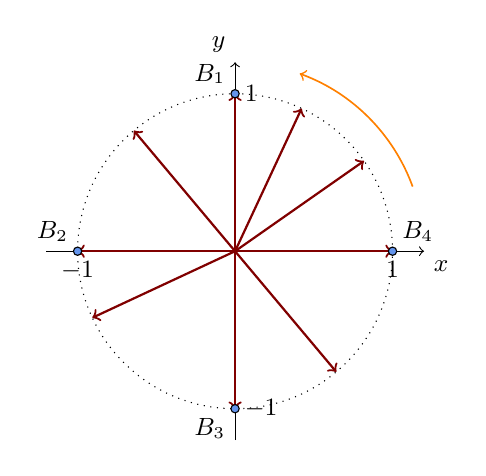
\begin{tikzpicture}[x=20mm,y=20mm, font=\small]
\begin{scope}[->]
\draw (-1.2,0) -- (1.2,0) node [below right] {$x$};
\draw (0,-1.2) -- (0,1.2) node [above left] {$y$};
\end{scope}

\foreach \x/\xtext in {-1/-1,1/1}
\node[below] at(\x,0) {$\xtext$};

\foreach \xi in {-1,1}
\draw (\xi,1.5pt) -- (\xi,-1.5pt);

\foreach \yi in {-1,1}
\draw(1.5pt,\yi)--(-1.5pt,\yi);

\foreach \y/\ytext in {-1/-1,1/1}
\node[right] at(0,\y) {$\ytext$};

\begin{scope}[Maroon, thick, ->]
\foreach \z in {0,35,65,90,130,180,205,270,310}
\draw[rotate=\z] (0,0)--(1,0 );
\end{scope}
\draw[dotted] (0,0) circle (1);

\node [above left] at (0,1) {$B_1$};
\node [above left] at (-1,0) {$B_2$};
\node [below left] at (0,-1) {$B_3$};
\node [above right] at (1,0) {$B_4$};

\draw[->,semithick, orange] (20:1.2) arc[radius=1.2, start angle=20, end angle=70];
\begin{scope}[fill=CornflowerBlue, draw=black]
\filldraw (1,0) circle (1.5pt);
\filldraw (0,1) circle (1.5pt);
\filldraw (-1,0) circle (1.5pt);
\filldraw (0,-1) circle (1.5pt);
\end{scope}
\end{tikzpicture}

\end{center}
\end{multicols}


\begin{definizione}
La componente orizzontale $u_{x}$ del vettore unitario inclinato dell'angolo~$\alpha$ rispetto all'asse~$x$, si chiama \emph{coseno dell'angolo
$\alpha$}, in simboli~$u_{x}=\cos(\alpha)$. Chiamiamo \emph{seno dell'angolo ${\alpha}$} la componente verticale $u_{y}$
del vettore unitario inclinato dell'angolo~${\alpha}$ rispetto all'asse~$x$, in simboli~$u_{y}=\sin(\alpha)$.
Scriviamo~$\vec{u}=(\cos(\alpha);\sin(\alpha))$ o anche~$B(\cos(\alpha);\sin(\alpha))$.
\end{definizione}

Confrontando questa definizione con quanto descritto sopra possiamo innanzitutto affermare che seno e coseno di un angolo sono numeri reali
positivi, negativi o nulli a seconda dell'angolo formato dal vettore e quindi della posizione del punto~$B$ sulla circonferenza:
\begin{itemize*}
\item se~$\alpha=0\grado \:\Rightarrow\: B(1;0) \:\Rightarrow\: \vec{u}=(\cos(0\grado);\sin (0\grado)) \:\Rightarrow\: \cos(0\grado)=1$ e~$\sin(0\grado)=0$;
\item se~$\alpha=90\grado \:\Rightarrow\: B(0;1) \:\Rightarrow\: \vec{u}=(\cos(90\grado);\sin(90\grado)) \:\Rightarrow\: \cos(90\grado)=0$ e~$\sin(90\grado)=1$;
\item se~$\alpha=180\grado \:\Rightarrow\: B(-1;0) \:\Rightarrow\: \vec{u}=(\cos(180\grado);\sin(180\grado)) \:\Rightarrow\: \cos(180\grado)=-1$ e~$\sin(180\grado)=0$;
\item se~$\alpha=270\grado \:\Rightarrow\: B(0;-1) \:\Rightarrow\: \vec{u}=(\cos(270\grado);\sin(270\grado)) \:\Rightarrow\: \cos(270\grado)=0$ e~$\sin(270\grado)=-1$;
\item se~$\alpha=360\grado \:\Rightarrow\: B(1;0) \:\Rightarrow\: \vec{u}=(\cos(360\grado)$;$\sin (360\grado)) \:\Rightarrow\: \cos(360\grado)=1$ e~$\sin(360\grado)=0$.
\end{itemize*}

Per alcuni valori intermedi dell'angolo è possibile calcolare i relativi valori di seno e coseno usando metodi geometrici, per altri valori si può far uso
della calcolatrice scientifica.
Comunque, dai risultati sopra ottenuti, soprattutto riguardando la figura, possiamo affermare che qualunque sia l'angolo $\alpha$ sono sempre verificate le disuguaglianze:
$-1\le\sin(\alpha)\le~1$ e~$-1\le\cos(\alpha)\le~1$.

Ci proponiamo ora di tracciare il grafico della funzione~$y = \sin(x)$. A questo scopo fermiamo la rotazione del vettore unitario ogni
$30\grado$ (completate il disegno) e segniamo sulla circonferenza i punti~$B_0$, $B_1$, $B_2$, ecc.
\begin{center}
 % (c) 2012 Dimitrios Vrettos - d.vrettos@gmail.com

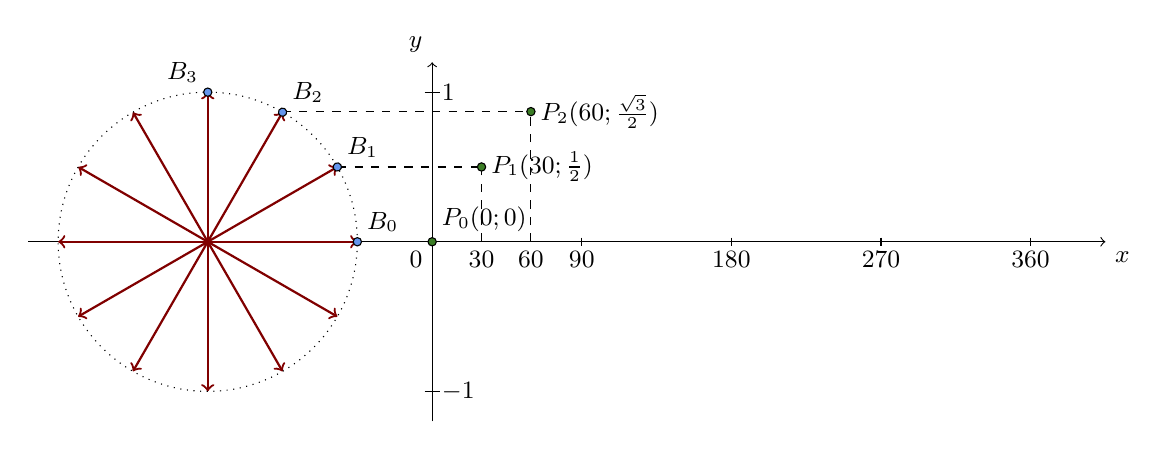
\begin{tikzpicture}[x=19mm,y=19mm, font=\small]
\begin{scope}[->]
\draw (-1.2,0) -- (6,0) node [below right] {$x$};
\draw (1.5,-1.2) -- (1.5,1.2) node [above left] {$y$};
\end{scope}

\node[below left] at (1.5,0) {0};
\foreach \x/\xtext in {1.83/30\grado,2.16/60\grado,2.5/90\grado,3.5/180\grado,4.5/270\grado,5.5/360\grado}
\node[below] at(\x,0) {$\xtext$};

\foreach \xi in {2.5,3.5,4.5,5.5}
\draw (\xi,1.5pt) -- (\xi,-1.5pt);

\foreach \yi in {-1,1}
\draw (1.45,\yi) -- (1.55,\yi);

\foreach \y/\xtext in {-1/-1,1/1}
\node[right] at(1.5,\y) {$\xtext$};

\begin{scope}[Maroon, thick, ->]
\foreach \z in {0,30,60,90,120,150,180,210,240,270,300,330}
\draw[rotate=\z] (0,0)--(1,0);
\end{scope}

\draw[dotted] (0,0) circle (1);
\node [above left] at (0,1) {$B_3$};
\node [above right] at (1,0) {$B_0$};

\begin{scope}[dashed]
\draw(.87,.5)--(1.83,.5);
\draw (1.83,0) -- (1.83,.5);
\draw (0.5,0.87) -- (2.16,0.87);
\draw (2.16,0) -- (2.16,0.87);
\end{scope}
\begin{scope}[fill=CornflowerBlue, draw=black]
\filldraw (1,0) circle (1.5pt);
\filldraw[rotate=30] (1,0) circle (1.5pt) node (B1)[above right] {$B_1$};
\filldraw[rotate=60] (1,0) circle (1.5pt) node (B2)[above right] {$B_2$};
\filldraw (0,1) circle (1.5pt);
\end{scope}

\begin{scope}[fill=OliveGreen, draw=black]
\filldraw (1.5,0) circle (1.5pt)node [above right] {$P_0(0\grado;0)$};
\filldraw (1.83,.5) circle (1.5pt)node [right] {$P_1(30\grado;\frac{1}{2})$};
\filldraw (2.16,.87) circle (1.5pt)node [right] {$P_2(60\grado;\frac{\sqrt{3}}{2})$};
\end{scope}
\end{tikzpicture}
\end{center}


Accanto alla rotazione del vettore unitario abbiamo tracciato un riferimento cartesiano dove sull'asse~$x$ riportiamo le misure in gradi
degli angoli descritti dal vettore unitario e sull'asse~$y$ i valori assunti da $\sin(x)$, cioè dall'ordinata dell'estremo libero
del vettore unitario che ruota in senso antiorario.

Per ogni angolo~$x$ descritto riporteremo nel riferimento cartesiano~$\sin(x)$. Il punto~$B_0$ ha ordinata nulla dunque il primo punto che
dobbiamo segnare nel riferimento cartesiano per costruire il grafico di~$y=\sin(x)$ è l'origine; per segnare il punto di coordinate
$P_1(30\grado$; $\sin(30\grado))$, da~$B_1$ tracciamo la parallela all'asse~$x$ fino ad incontrare la parallela all'asse~$y$ tracciata da~$30\grado$.
Proseguite in questo modo per tutti gli altri punti $B_i$ della circonferenza per determinare i rispettivi punti $P_i$. Unendo i punti $P_i$ trovati si ha il grafico
della funzione~$y = \sin(x)$.

Noi l'abbiamo tracciato con \emph{GeoGebra}\footnote{un particolare software di matematica dinamica per la didattica (\url{http://www.geogebra.org}).}. Notiamo che il valore massimo~$1$ si ha per l'angolo di~$90\grado$ mentre il minimo~$-1$ si ha
per l'angolo di~$270\grado$. Se il vettore unitario dopo un giro completo ricominciasse nuovamente a ruotare in senso antiorario (positivo),
descrivendo angoli maggiori di~$360\grado$, il grafico si ripeterebbe identico al tratto compreso tra~$0\grado$ e~$360\grado$.
Per questo motivo diciamo che la funzione~$y= \sin(x)$ ha un andamento periodico.
\begin{center}
 % (c) 2012 Dimitrios Vrettos - d.vrettos@gmail.com

\begin{tikzpicture}[x=15mm,y=15mm, font=\small,]
\begin{scope}[->]
\draw (-.8,0) -- (7,0) node [below right] {$x$};
\draw (0,-1.2) -- (0,1.2) node [above left] {$y$};
\end{scope}

\foreach \xi in {1.573,3.145,4.718,6.291}
\draw (\xi,1.5pt) -- (\xi,-1.5pt);

\foreach \yi in {-1,1}
\draw (-1.5pt,\yi) -- (1.5pt,\yi);

\begin{scope}[dotted]
\draw (1.573,0) -- (1.573,1);
\draw (4.718,0) -- (4.718,-1);
\draw (-.8,1) -- (6.5,1);
\draw (-.8,-1) -- (6.5,-1);

\end{scope}
\draw[color=blue, domain=-.8:6.5,smooth]
plot[id=sin] function{sin(x)};
\node[below left] at (0,0) {$0\grado$};
\foreach \x/\xtext in {1.573/90\grado,3.145/180\grado,4.718/270\grado,6.291/360\grado}
\node[below] at(\x,0) {$\xtext$};

\node[above right] at(0,1) {$1$};
\node[below right] at(0,-1) {$-1$};

\end{tikzpicture}
\end{center}


Abbiamo tracciato anche il grafico della funzione~$y=\cos(x)$; sfruttando quanto fatto all'inizio del paragrafo;
lasciamo al lettore di segnare sul grafico i valori dell'angolo per cui il coseno è nullo, il valore per cui il coseno
assume il valore minimo~$-1$, il punto del grafico di ascissa~$=360\grado$.
Per lo stesso discorso fatto sopra possiamo dire che la funzione~$y=\cos(x)$ ha un andamento periodico.
\begin{center}
 % (c) 2012 Dimitrios Vrettos - d.vrettos@gmail.com

\begin{tikzpicture}[x=15mm,y=15mm, font=\small,]
\begin{scope}[->]
\draw (-.8,0) -- (7,0) node [below right] {$x$};
\draw (0,-1.2) -- (0,1.2) node [above left] {$y$};
\end{scope}

\foreach \xi in {1.573,3.145,4.718,6.291}
\draw (\xi,1.5pt) -- (\xi,-1.5pt);

\foreach \yi in {-1,1}
\draw (-1.5pt,\yi) -- (1.5pt,\yi);

\begin{scope}[dotted]
\draw (-.8,1) -- (6.5,1);
\draw (-.8,-1) -- (6.5,-1);
\draw (3.1415,0) -- (3.1415,-1);
\draw (6.2831,0) -- (6.2831,1);

\end{scope}
\draw[color=blue, domain=-.8:6.5,smooth]
plot[id=sin] function{cos(x)};
\node[below left] at (0,0) {$0\grado$};
\foreach \x/\xtext in {1.573/90\grado,3.145/180\grado,4.718/270\grado,6.291/360\grado}
\node[below] at(\x,0) {$\xtext$};

\node[above right] at(0,1) {$1$};
\node[below right] at(0,-1) {$-1$};

\end{tikzpicture}
\end{center}

\newpage
% (c) 2012 Silvia Cibola - silvia.cibola@gmail.com
% (c) 2012-2014 Dimitrios Vrettos - d.vrettos@gmail.com

\section{Esercizi}

\subsection{Esercizi dei singoli paragrafi}

\subsubsection*{C.2 - Rappresentazione di una corrispondenza}

\begin{esercizio}
\label{ese:C.1}
Rappresenta con un grafico cartesiano la corrispondenza~$\Kor$: ``essere nato nell'anno'' di dominio l'insieme~$A=\{$Galileo, Napoleone, Einstein, Fermi, Obama$\}$
e codominio l'insieme~$B=\{$1901, 1564, 1961, 1879, 1769, 1920, 1768$\}$. Rappresenta per elencazione il sottoinsieme~$G_\Kor$ del prodotto cartesiano~$A \times B$.
Stabilisci infine gli elementi dell'immagine~$\IM$.
\end{esercizio}

\begin{esercizio}
\label{ese:C.2}
L'insieme~$S=\{$casa, volume, strada, ufficio, clavicembalo, cantautore, assicurazione$\}$ è il codominio della corrispondenza~$\Kor$: ``essere il numero di sillabe di'' il cui dominio
è~$X=\{x \in\insN \mid  0<x<10\}$. Rappresenta con un grafico cartesiano la corrispondenza assegnata, evidenzia, come nell'esempio~\ref{ex:C.1} a pagina~\pageref{ex:C.1}, l'insieme~$G_\Kor$,
scrivi per elencazione l'insieme~$\IM$.
\end{esercizio}

\begin{esercizio}
\label{ese:C.3}
Completa la rappresentazione con grafico sagittale della corrispondenza $\Kor$ ``essere capitale di''. La freccia che collega gli elementi del dominio $\Dom$ con quelli del codominio $\Cod$ rappresenta
il predicato~$\Kor$.
\begin{center}
 % (c) 2012 Dimitrios Vrettos - d.vrettos@gmail.com
\begin{tikzpicture}[x=10mm, y=10mm]

\node[ellipse, minimum height=3cm,draw, minimum width=4cm] (D) at (0,0) {};

\node[above] (D1) at (D.north) {$\Dom$};

\begin{scope}[fill=CornflowerBlue]

\filldraw (.7,1) circle (2pt) node (a) {};
\node[left] at (.7,1) {Roma};
\filldraw (1,.2) circle (2pt) node (b) {};
\node[left] at (1,.2) {Parigi};

\filldraw (-1.3,-.5) circle (2pt) node (c) {};
\end{scope}

\begin{scope}[xshift=5cm]
\node[ellipse, minimum height=3cm,draw, minimum width=4cm] (C) at (0,0) {};

\node[above] (C1) at (C.north) {$\Cod$};

\begin{scope}[fill=LimeGreen]
\filldraw (-.1,1) circle (2pt) node (a1) {};
\filldraw (-.2,.2) circle (2pt)node (b1) {};
\filldraw (.2,-.8) circle (2pt) node (c1) {};

\node[right]  at (-.1,1) {Francia};
\node[right]  at (.2,-.8) {Italia};
\node[right] at (-.2,.2) {Grecia};

\end{scope}
\end{scope}
\begin{scope}[->,smooth,thick]
\draw[red] (c) .. controls +(-30:2cm) and +(-180:2cm) .. (b1);
\end{scope}
\end{tikzpicture}
\end{center}

\end{esercizio}

\subsubsection*{C.3 - Caratteristiche di una corrispondenza}
\begin{esercizio}
\label{ese:C.4}
\`E univoca la corrispondenza~$\Kor$ definita tra l'insieme~$P= \{$parola del proverbio ``rosso di sera, bel tempo si spera''$\}$ e l'insieme~$A=\{$lettere dell'alfabeto italiano$\}$
che associa ad ogni parola la sua iniziale? Ti sembra corretto affermare che dominio $\Dom$ e insieme di definizione $\ID$ coincidono? Completa con il simbolo corretto
la relazione tra insieme immagine e codominio:~$\IM\ldots\Cod$. Fai il grafico sagittale della corrispondenza.
\end{esercizio}

\begin{esercizio}
\label{ese:C.5}
$\Kor$ è la corrispondenza tra l'insieme ~$\insN$ dei naturali e l'insieme degli interi relativi~$\insZ$ espressa dal predicato ``essere il quadrato di''. Ti sembra corretto affermare che
dominio $\Dom$ e insieme di definizione $\ID$ coincidono? Perché~$\IM=\Cod$? La corrispondenza è univoca?
\end{esercizio}

\pagebreak

\begin{esercizio}
\label{ese:C.6}
Una corrispondenza~$\Kor$ è assegnata con il suo grafico cartesiano.
\begin{center}
 % (c) 2012 Dimitrios Vrettos - d.vrettos@gmail.com
\begin{tikzpicture}[x=10mm, y=10mm]

\begin{scope}[->]
\draw (-.5,0) -- (12,0);
\draw (0,-.5) -- (0,7);
\end{scope}

\foreach \x in {1,2,...,11}
\draw (\x,1.5pt) -- (\x,-1.5pt);

\foreach \y in {1,2,...,6}
\draw (1.5pt,\y) -- (-1.5pt,\y);

\foreach \xi/\xtext in {1/A,2/B,3/C,4/D,5/E,6/F,7/G,8/H,9/I,10/L,11/M}
\node[below] at (\xi,0) {$\xtext$};

\foreach \yi/\ytext in {1/1,2/2,3/3,4/4,5/5,6/6}
\node[left] at (0,\yi){\ytext};

\draw[orange, dotted] (0,0) grid (11,6);

\begin{scope}[fill=CornflowerBlue]
\foreach \x in {1,6}
\filldraw (\x,1) circle (2pt);

\foreach \x in {2,5,8}
\filldraw (\x,2) circle (2pt);

\foreach \x in {4,10}
\filldraw (\x,4) circle (2pt);

\filldraw (3,5) circle (2pt);
\filldraw (11,6) circle (2pt);
\end{scope}
\end{tikzpicture}
\end{center}
Completa e rispondi alle domande:

\begin{enumeratea}
\item $\Dom=$\{\dotfill\};
\item $\Cod=$\{\dotfill\};
\item $\ID=$\{\dotfill\};
\item $\IM=$\{\dotfill\};
\item la corrispondenza è biunivoca?
\item di quali elementi dell'insieme di definizione 2 ne è l'immagine?
\item quale elemento del codominio è l'immagine di~$M$?
\end{enumeratea}
\end{esercizio}

%\newpage
\begin{esercizio}
\label{ese:C.7}
I tre grafici sagittali rappresentano altrettante corrispondenze, $\Kor_1$, $\Kor_2$, $\Kor_3$.
Completa per ciascuna di esse la descrizione schematizzata nel riquadro sottostante:
\begin{center}
 % (c) 2012 Dimitrios Vrettos - d.vrettos@gmail.com
\begin{tikzpicture}[x=10mm, y=10mm]

\node[circle, minimum height=2cm,draw] (A) at (0,0) {};

\node[above] (A1) at (A.north) {$A$};

\begin{scope}[fill=CornflowerBlue]

\filldraw (.5,.5) circle (2pt) node (a) {};
\node[left] at (.5,.5) {1};
\filldraw (.8,.2) circle (2pt) node (b) {};
\node[left] at (.8,.2) {2};
\filldraw (-.4,-.5) circle (2pt) node (c) {};
\node[left] at (-.4,-.5)  {3};
\filldraw (-.5,0) circle (2pt);
\node[left] at (-.5,0)  {4};
\filldraw (-.3,.5) circle (2pt);
\node[left] at (-.3,.5)  {5};
\end{scope}

\begin{scope}[xshift=2.3cm]
\node[circle, minimum height=2cm,draw] (B) at (0,0) {};

\node[above] (B1) at (B.north) {$B$};

\begin{scope}[fill=LimeGreen]
\filldraw (-.1,.6) circle (2pt) node (a1) {};
\filldraw (-.2,.2) circle (2pt)node (b1) {};
\filldraw (.2,-.7) circle (2pt) node (c1) {};
\filldraw(.5,-.2) circle (2pt);

\node[right]  at (-.1,.6) {$a$};
\node[right] at (-.2,.2) {$b$};
\node[right]  at (.2,-.7) {$c$};
\node[right] at (.5,-.2) {$d$};
\end{scope}
\end{scope}

\begin{scope}[->,smooth,thick]
\draw[Maroon] (a) .. controls +(30:1cm) and +(150:.5cm) .. (a1);
\draw[purple] (b) .. controls +(30:.5cm) and +(180:0.5cm) .. (b1);
\draw[orange] (c) .. controls +(30:1cm) and +(-90:1cm) .. (b1);
\draw[orange] (c) .. controls +(30:1cm) and +(-180:2cm) .. (c1);
\end{scope}

\begin{scope}[yshift=-2.5cm]
\matrix (m) [matrix of nodes]
{$\Dom=$&\ldots\\
$\Cod=$&\ldots\\
$\ID=$&\ldots\\
$\IM=$&\ldots\\
Tipo$=$&\ldots\\};
\end{scope}


\begin{scope}[xshift=4.6cm]

\node[circle, minimum height=2cm,draw] (A) at (0,0) {};

\node[above] (A1) at (A.north) {$A$};

\begin{scope}[fill=CornflowerBlue]

\filldraw (0,.7) circle (2pt) node (a) {};
\node[left] at (0,.7) {$a$};
\filldraw (.7,0) circle (2pt) node (b) {};
\node[left] at (.7,0) {$b$};
\filldraw (-.4,-.5) circle (2pt) node (c) {};
\node[left] at (-.4,-.5)  {$c$};
\end{scope}

\begin{scope}[xshift=2.3cm]
\node[circle, minimum height=2cm,draw] (B) at (0,0) {};

\node[above] (B1) at (B.north) {$B$};

\begin{scope}[fill=LimeGreen]
\filldraw (-.1,.6) circle (2pt) node (a1) {};
\filldraw (-.2,.2) circle (2pt)node (b1) {};
\filldraw (.2,-.7) circle (2pt) node (c1) {};

\node[right]  at (-.1,.6) {$m$};
\node[right] at (-.2,.2) {$n$};
\node[right]  at (.2,-.7) {$p$};
\end{scope}
\end{scope}

\begin{scope}[->,smooth,thick]
\draw[Maroon] (a) .. controls +(30:1cm) and +(180:1cm) .. (b1);
\draw[purple] (b) .. controls +(30:1cm) and +(180:1cm) .. (c1);
\draw[orange] (c) .. controls +(30:.5cm) and +(-180:2cm) .. (a1);
\end{scope}

\begin{scope}[yshift=-2.5cm]
\matrix (m) [matrix of nodes]
{$\Dom=$&\ldots\\
$\Cod=$&\ldots\\
$\ID=$&\ldots\\
$\IM=$&\ldots\\
Tipo$=$&\ldots\\};
\end{scope}
\end{scope}

\begin{scope}[xshift=9.2cm]
\node[circle, minimum height=2.cm,draw] (A) at (0,0) {};

\node[above] (A1) at (A.north) {$A$};

\begin{scope}[fill=CornflowerBlue]

\filldraw (.3,.7) circle (2pt) node (a) {};
\node[left] at (.3,.7) {1};
\filldraw (.6,.2) circle (2pt) node (b) {};
\node[left] at (.6,.2) {2};
\filldraw (-.3,-.5) circle (2pt) node (c) {};
\node[left] at (-.3,-.5)  {3};
\filldraw (-.5,0) circle (2pt) node (d){};
\node[left] at (-.5,0)  {4};

\end{scope}

\begin{scope}[xshift=2.3cm]
\node[circle, minimum height=2cm,draw] (B) at (0,0) {};

\node[above] (B1) at (B.north) {$B$};

\begin{scope}[fill=LimeGreen]
\filldraw (-.1,.6) circle (2pt) node (a1) {};
\filldraw (-.2,.2) circle (2pt)node (b1) {};
\filldraw (.1,-.8) circle (2pt) node (c1) {};
\filldraw(.5,-.1) circle (2pt) node (d1) {};
\filldraw(-.7,-.4) circle (2pt) node (e1) {};

\node[right]  at (-.1,.6) {$a$};
\node[right] at (-.2,.2) {$b$};
\node[right]  at (.1,-.8) {$c$};
\node[right] at (.5,-.1) {$d$};
\node[right] at (-.7,-.4) {$e$};
\end{scope}
\end{scope}

\begin{scope}[->,smooth,thick]
\draw[Maroon] (a) .. controls +(30:.5cm) and +(90:.5cm) .. (e1);
\draw[purple] (b) .. controls +(30:.5cm) and +(90:.5cm) .. (e1);
\draw[orange] (c) .. controls +(30:.5cm) and +(-180:2cm) .. (b1);
\draw[red] (d) .. controls +(-30:2cm) and +(-120:1cm) .. (d1);
\end{scope}

\begin{scope}[yshift=-2.5cm]
\matrix (m) [matrix of nodes]
{$\Dom=$&\ldots\\
$\Cod=$&\ldots\\
$\ID=$&\ldots\\
$\IM=$&\ldots\\
Tipo$=$&\ldots\\};
\end{scope}
\end{scope}
\end{tikzpicture}
\end{center}
\end{esercizio}
\pagebreak
\begin{esercizio}
\label{ese:C.8}
Il dominio della corrispondenza~$\Kor$ è l'insieme~$\insZ\times\insZ$ e~$\insZ$ ne è il codominio; l'immagine della coppia~$(a;b)$ è l'intero~$p=a \cdot b$.
\begin{enumeratea}
\item Stabilisci l'insieme di definizione $\ID$ e l'insieme immagine $\IM$;
\item perché questa corrispondenza non è biunivoca?
\item tutte le coppie aventi almeno un elemento uguale a zero hanno come immagine \ldots;
\item 1 è l'immagine di \ldots;
\item se gli elementi della coppia sono numeri concordi, allora l'immagine è \ldots;
\item un numero negativo è immagine di \ldots
\end{enumeratea}
Fai degli esempi che illustrino le tue affermazioni precedenti.
\end{esercizio}

\begin{esercizio}
\label{ese:C.9}
Il dominio $\Dom$ della corrispondenza~$\Kor$ è l'insieme~$\insZ\times\insZ$ e~$\insZ$ ne è il codominio $\Cod$; l'immagine della coppia~$(a;b)$ è il numero razionale~$q=\frac{a}{b}$.
\begin{enumeratea}
\item Stabilisci l'insieme di definizione $\ID$ e l'insieme immagine $\IM$;
\item completa:
\begin{enumeratea}
\item lo zero è immagine delle coppie \ldots;
\item se gli elementi della coppia sono numeri opposti l'immagine è \ldots;
\item se gli elementi della coppia sono numeri concordi allora l'immagine è \ldots;
\item un numero negativo è immagine di \ldots
\end{enumeratea}
\item fai degli esempi che illustrino le tua affermazioni precedenti.
\end{enumeratea}
\end{esercizio}

\begin{esercizio}
\label{ese:C.10}
In un gruppo di~10 persone, due si erano laureate in medicina e tre in legge nell'anno~1961, mentre quattro anni dopo, una si era laureata in fisica, un'altra in scienze e due in legge.
Considerate i seguenti insiemi:~$P=\{x \mid  x$ è una persona del gruppo$\}$; $A=\{$1960, 1961, 1964, 1965$\}$; $F=\{x \mid  x$ è una facoltà universitaria$\}$.
Fatene la rappresentazione con diagramma di Eulero-Venn e studiate le corrispondenze~$\Kor_1$, $\Kor_2$, espresse dai predicati:~$\Kor_1$: ``essersi laureato nell'anno'' e~$K_2$:
``essere laureato in'', mettendo in evidenza per ciascuna dominio, codominio, insieme di definizione, immagine, tipo.

Completate:
\begin{enumeratea}
\item nel gruppo ci sono \ldots persone laureate in legge, di cui \ldots nell'anno~1961 e le altre \ldots nell'anno \ldots;
\item nel~1961 si sono laureate \ldots di cui \ldots in medicina;
\item negli anni \ldots non si è laureata nessuna persona del gruppo considerato;
\item tra le~10 persone \ldots non si è laureata.
\end{enumeratea}
N.B.: ciascuno possiede una sola laurea.

Maria si è laureata in fisica nello stesso anno in cui si è laureato suo marito Luca; Andrea, fratello di Luca, non è medico, ha frequentato una facoltà diversa da quella del fratello
e si è laureato in un anno diverso. Supponendo che Maria, Luca e Andrea siano tra le~10 persone di cui sopra, completate:

Maria si è laureata nell'anno \ldots. Andrea si è laureato nell'anno \ldots in \ldots. Luca si è laureato nell'anno \ldots in \ldots
\end{esercizio}

\cleardoublepage
